\documentclass{article}

  % packages
    % basic stuff for rendering math
    \usepackage[letterpaper, top=1in, bottom=1in, left=1in, right=1in]{geometry}
    \usepackage[utf8]{inputenc}
    \usepackage[english]{babel}
    \usepackage{amsmath} 
    \usepackage{amssymb}

    % extra math symbols and utilities
    \usepackage{mathtools}        % for extra stuff like \coloneqq
    \usepackage{mathrsfs}         % for extra stuff like \mathsrc{}
    \usepackage{centernot}        % for the centernot arrow 
    \usepackage{bm}               % for better boldsymbol/mathbf 
    \usepackage{enumitem}         % better control over enumerate, itemize
    \usepackage{hyperref}         % for hypertext linking
    \usepackage{fancyvrb}          % for better verbatim environments
    \usepackage{newverbs}         % for texttt{}
    \usepackage{xcolor}           % for colored text 
    \usepackage{listings}         % to include code
    \usepackage{lstautogobble}    % helper package for code
    \usepackage{parcolumns}       % for side by side columns for two column code
    

    % page layout
    \usepackage{fancyhdr}         % for headers and footers 
    \usepackage{lastpage}         % to include last page number in footer 
    \usepackage{parskip}          % for no indentation and space between paragraphs    
    \usepackage[T1]{fontenc}      % to include \textbackslash
    \usepackage{footnote}
    \usepackage{etoolbox}

    % for custom environments
    \usepackage{tcolorbox}        % for better colored boxes in custom environments
    \tcbuselibrary{breakable}     % to allow tcolorboxes to break across pages

    % figures
    \usepackage{pgfplots}
    \pgfplotsset{compat=1.18}
    \usepackage{float}            % for [H] figure placement
    \usepackage{tikz}
    \usepackage{tikz-cd}
    \usepackage{circuitikz}
    \usetikzlibrary{arrows}
    \usetikzlibrary{positioning}
    \usetikzlibrary{calc}
    \usepackage{graphicx}
    \usepackage{algorithmic}
    \usepackage{caption} 
    \usepackage{subcaption}
    \captionsetup{font=small}

    % for tabular stuff 
    \usepackage{dcolumn}

    \usepackage[nottoc]{tocbibind}
    \pdfsuppresswarningpagegroup=1
    \hfuzz=5.002pt                % ignore overfull hbox badness warnings below this limit

  % New and replaced operators
    \DeclareMathOperator*{\argmin}{\arg\!\min}
    \DeclareMathOperator*{\argmax}{\arg\!\max}
    \newcommand{\qed}{\hfill$\blacksquare$}     % I like QED squares to be black

  % Custom Environments
    \newtcolorbox[auto counter, number within=section]{question}[1][]
    {
      colframe = orange!25,
      colback  = orange!10,
      coltitle = orange!20!black,  
      breakable, 
      title = \textbf{Question \thetcbcounter ~(#1)}
    }

    \newtcolorbox[auto counter, number within=section]{exercise}[1][]
    {
      colframe = teal!25,
      colback  = teal!10,
      coltitle = teal!20!black,  
      breakable, 
      title = \textbf{Exercise \thetcbcounter ~(#1)}
    }
    \newtcolorbox[auto counter, number within=section]{solution}[1][]
    {
      colframe = violet!25,
      colback  = violet!10,
      coltitle = violet!20!black,  
      breakable, 
      title = \textbf{Solution \thetcbcounter}
    }
    \newtcolorbox[auto counter, number within=section]{lemma}[1][]
    {
      colframe = red!25,
      colback  = red!10,
      coltitle = red!20!black,  
      breakable, 
      title = \textbf{Lemma \thetcbcounter ~(#1)}
    }
    \newtcolorbox[auto counter, number within=section]{theorem}[1][]
    {
      colframe = red!25,
      colback  = red!10,
      coltitle = red!20!black,  
      breakable, 
      title = \textbf{Theorem \thetcbcounter ~(#1)}
    } 
    \newtcolorbox[auto counter, number within=section]{proposition}[1][]
    {
      colframe = red!25,
      colback  = red!10,
      coltitle = red!20!black,  
      breakable, 
      title = \textbf{Proposition \thetcbcounter ~(#1)}
    } 
    \newtcolorbox[auto counter, number within=section]{corollary}[1][]
    {
      colframe = red!25,
      colback  = red!10,
      coltitle = red!20!black,  
      breakable, 
      title = \textbf{Corollary \thetcbcounter ~(#1)}
    } 
    \newtcolorbox[auto counter, number within=section]{proof}[1][]
    {
      colframe = orange!25,
      colback  = orange!10,
      coltitle = orange!20!black,  
      breakable, 
      title = \textbf{Proof. }
    } 
    \newtcolorbox[auto counter, number within=section]{definition}[1][]
    {
      colframe = yellow!25,
      colback  = yellow!10,
      coltitle = yellow!20!black,  
      breakable, 
      title = \textbf{Definition \thetcbcounter ~(#1)}
    } 
    \newtcolorbox[auto counter, number within=section]{example}[1][]
    {
      colframe = blue!25,
      colback  = blue!10,
      coltitle = blue!20!black,  
      breakable, 
      title = \textbf{Example \thetcbcounter ~(#1)}
    } 
    \newtcolorbox[auto counter, number within=section]{code}[1][]
    {
      colframe = green!25,
      colback  = green!10,
      coltitle = green!20!black,  
      breakable, 
      title = \textbf{Code \thetcbcounter ~(#1)}
    } 
    \newtcolorbox[auto counter, number within=section]{algo}[1][]
    {
      colframe = green!25,
      colback  = green!10,
      coltitle = green!20!black,  
      breakable, 
      title = \textbf{Algorithm \thetcbcounter ~(#1)}
    } 

    \BeforeBeginEnvironment{example}{\savenotes}
    \AfterEndEnvironment{example}{\spewnotes}
    \BeforeBeginEnvironment{lemma}{\savenotes}
    \AfterEndEnvironment{lemma}{\spewnotes}
    \BeforeBeginEnvironment{theorem}{\savenotes}
    \AfterEndEnvironment{theorem}{\spewnotes}
    \BeforeBeginEnvironment{corollary}{\savenotes}
    \AfterEndEnvironment{corollary}{\spewnotes}
    \BeforeBeginEnvironment{proposition}{\savenotes}
    \AfterEndEnvironment{proposition}{\spewnotes}
    \BeforeBeginEnvironment{definition}{\savenotes}
    \AfterEndEnvironment{definition}{\spewnotes}
    \BeforeBeginEnvironment{exercise}{\savenotes}
    \AfterEndEnvironment{exercise}{\spewnotes}
    \BeforeBeginEnvironment{proof}{\savenotes}
    \AfterEndEnvironment{proof}{\spewnotes}
    \BeforeBeginEnvironment{solution}{\savenotes}
    \AfterEndEnvironment{solution}{\spewnotes}
    \BeforeBeginEnvironment{question}{\savenotes}
    \AfterEndEnvironment{question}{\spewnotes}
    \BeforeBeginEnvironment{code}{\savenotes}
    \AfterEndEnvironment{code}{\spewnotes}
    \BeforeBeginEnvironment{algo}{\savenotes}
    \AfterEndEnvironment{algo}{\spewnotes}

    \definecolor{dkgreen}{rgb}{0,0.6,0}
    \definecolor{gray}{rgb}{0.5,0.5,0.5}
    \definecolor{mauve}{rgb}{0.58,0,0.82}
    \definecolor{darkblue}{rgb}{0,0,139}
    \definecolor{lightgray}{gray}{0.93}
    \renewcommand{\algorithmiccomment}[1]{\hfill$\triangleright$\textcolor{blue}{#1}}

    % default options for listings (for code)
    \lstset{
      autogobble,
      frame=ltbr,
      language=Python,
      aboveskip=3mm,
      belowskip=3mm,
      showstringspaces=false,
      columns=fullflexible,
      keepspaces=true,
      basicstyle={\small\ttfamily},
      numbers=left,
      firstnumber=1,                        % start line number at 1
      numberstyle=\tiny\color{gray},
      keywordstyle=\color{blue},
      commentstyle=\color{dkgreen},
      stringstyle=\color{mauve},
      backgroundcolor=\color{lightgray}, 
      breaklines=true,                      % break lines
      breakatwhitespace=true,
      tabsize=3, 
      xleftmargin=2em, 
      framexleftmargin=1.5em, 
      stepnumber=1
    }

  % Page style
    \pagestyle{fancy}
    \fancyhead[L]{Operating Systems}
    \fancyhead[C]{Muchang Bahng}
    \fancyhead[R]{Summer 2025} 
    \fancyfoot[C]{\thepage / \pageref{LastPage}}
    \renewcommand{\footrulewidth}{0.4pt}          % the footer line should be 0.4pt wide
    \renewcommand{\thispagestyle}[1]{}  % needed to include headers in title page

\begin{document}

\title{Operating Systems}
\author{Muchang Bahng}
\date{January 2024}

\maketitle
\tableofcontents
\pagebreak

  Up until now, we've seen the dynamics of how one program works in a computer system. The code, which first resides in the disk, is fetched (through blocks) into memory, and after compiling (precomiling, compiling, assembling, linking), we have a binary. The binary is then loaded into memory in the stack frame, and the CPU executes the instructions. The CPU also has a cache, which stores the most frequently accessed data during the process, taking advantage of locality for efficiency. 

  Our computer obvious does not just run one program. It runs several, and to run several, we need some control mechanism to manage how these programs interact with the CPU, memory, and disk. For example, one problem is that if we download application A and application B and run their binaries, how do we know whether they share memory addresses and consequently overwrite each other's data?\footnote{This is different from linking, where we have relocation tables to ensure that \textit{object files} do not conflict with each other.} The operating system takes care of these, which manages \textit{processes} that each have their own \textit{virtual memory space}. 

  Furthermore, consider some of the components of the computer: the RAM, disk, and IO devices like your keyboard and monitor. For security reasons, it is not wise to let the user applications (e.g. Chrome or Slack) control these devices completely. Their power must be restricted in some way. 
  \begin{enumerate}
    \item When you have a Chrome window and resize it, Chrome should not be able to modify the pixels outside that window. 
    \item When you want to print some statement using \texttt{printf}, 
    \item When you're editing a code file with VSCode, you want to limit the application to save to certain parts of the disk. 
    \item When you are running Chrome and Slack together, you don't want them to read each other's data directly. 
  \end{enumerate}
  This is also for convenience. Say that if you are creating an application that has the option to save files to disk, you don't want to write the hardware backend to write to the disk. You want to just call a function that writes to the disk, and the OS will take care of the rest. 

  \begin{definition}[Operating System]
    A common confusion is that people think that the \textbf{operating system} describes the computer itself, but it is really just another piece of software. What makes this piece of software so special is that it manages every other software in the computer. It provides generally three services: 
    \begin{enumerate}
      \item It \textbf{multiplexes} the hardware resources. Since there are many applications/programs with finite CPU resources (number of cores) and shared access to storage devices, the OS schedules some sharing mechanism for execution time on CPU cores and manages access to storage devices.
      \item It \textbf{abstracts} the hardware platform. Since each CPU core simply executes a sequence of instructions, the OS introduces processes and thread abstractions. Furthermore, it introduces \textit{filesystems} (file/directories) on top of raw storage devices. 
      \item It \textbf{protects} software principals from each other. Since many applications from various users are using the CPU, the OS provides isolation between them. It enforces user access permission (read/write) for files. 
    \end{enumerate}
  \end{definition}

  The OS is booted by the system firmware (BIOS or UEFI), which lives in ROM (sRAM and therefore non-volatile) and copies the OS from a fixed part of the disk, called the \textbf{bootloader}, into the RAM, which itself then loads the OS into memory. Once the OS starts running, it loads the rest of itself from disk, discovers and initializes hardware resources, and initializes its data structures and abstractions to make the system ready for users.

  \begin{definition}[Kernel]
    The \textbf{kernel} is the actual binary that is loaded into RAM that runs the OS. The kernel code and data resides in a fixed and protected range of addresses, called the \textbf{kernel space}, and user programs cannot access kernel space. 
  \end{definition}

\section{Process Management}

  \subsection{Control Flow}

    When we worked with jumps (conditional and unconditional), calls, and returns in assmebly, all of these operations were with respect to the \textbf{program state}, which is the isolated environment that the program is in. One program doesn't have any clue of what is going on anywhere else, such as other programs or input/output signals. This means that given what we have learned, 
    \begin{enumerate}
      \item programs cannot to write files to the disk (since that is outside the program). 
      \item programs cannot be terminated by pressing \texttt{CTRL + C} on the keyboard. 
      \item programs cannot receive data that arrives from the disk. 
      \item programs cannot send data to the monitor to display. 
      \item programs cannot react accordingly when there is an instruction to divide by $0$.\footnote{I guess you can use a conditional jump to check if the divisor is $0$ and then jump to a different part of the code.}
    \end{enumerate}
    To do all these things, we need to have access to the global \textbf{system state}, which the OS has access to. 

    It turns out that it is impossible for jumps and procedure calls to achieve this, and rather the system needs mechanisms for \textbf{exceptional control flow} (i.e. control flow that is not within the regular program state), or commonly referred to as \textbf{exceptions}. This requires the CPU to enter into a more powerful state than its current place in the program state, called the kernel state. The actual thing that triggers this is called an \textbf{interrupt}, which can come from both the hardware and software. In the kernel state, the CPU can access the hardware and perform operations that the program state cannot to handle these exceptions. 

    \begin{example}[Interrupts]
      Some examples of how the OS can be interrupted is: 
      \begin{enumerate}
        \item when one's WiFi card detects a signal. 
        \item a hard disk drive may interrupt the OS if a read fails due to a bad sector. 
        \item an application may request a system call to open a file. 
        \item If you have 10 applications running on 1 CPU core, you may want the CPU core to run to the next application every 10 milliseconds. So, there may be a system call every 10 milliseconds in each program to the OS to switch to the next application. 
      \end{enumerate}
    \end{example}

    \begin{definition}[Execution Modes]
      The CPU helps with this by providing two execution modes, which is determined by a special bit in the CPU called the \textbf{mode bit}. 
      \begin{enumerate}
        \item In \textbf{user mode}, the CPU executes only user-level instructions and accesses only the memory locations that the OS makes available to it. It also restricts which hardware components the CPU can directly access. 
        \item In \textbf{kernel mode}, the CPU executes any instructions and accesses any memory location (including those that store OS instructions and data). It can also directly access hardware components and execute special instructions. 
      \end{enumerate}
      Note that the execution mode is \textit{property of the CPU}!  
    \end{definition}

    \begin{example}[Monitor]
      A monitor is really just some device that scans a certain portion of memory at a certain frequency that is higher than the human eye can detect. In user mode, if you try to access this memory buffer, you get an exception. No user mode can access this memory buffer. 
    \end{example}

    \begin{example}[Amazon.com]
      When you are on Amazon to search up some product, you want to type in some keyword in the search bar. The web browser, say Chrome, that you are running it on, runs in user mode. When you type in the keyword, Chrome sends a system call to the OS, triggering the kernel mode which retrieves the keys that you pressed, and redirects it to Chrome. The same goes with the location of your mouse. When you move and click on a product, Chrome sends a system call to the OS, which then receives the mouse location and sends it back to Chrome. The application has no way to directly access the hardware. 
    \end{example}

    Now specifically, how does one enter in this kernel mode? We've already hinted at it before, but to elaborate, there are 4 types of exceptions. 

    \begin{definition}[Types of Exceptions/Interrupts]
      As we have mentioned, we go into kernel mode through exceptional control flows. To go back from the kernel mode to the user mode after the exception handling is done, the kernel must explicitly give back the control to the user program, which is done with a special instruction, which changes the CPU to the user mode again. At this point, it can return back to user mode at the current instruction, next instruction, or abort it. 
      \begin{enumerate}
        \item These control flows can either by \textbf{synchronous} (caused by an instruction) or \textbf{asynchronous} (caused by some other event external to the processor). Asynchronous interrupts are indicated by setting the processor's interrupt pins. 
        \item Furthermore, \textbf{intentional} exceptions transfer control to the OS to perform some function, and \textbf{unintentional} exceptions happen when there is a bug. 
      \end{enumerate}
      This gives us 4 categories of exceptions. 
      \begin{enumerate}
        \item Intentional synchronous exceptions are \textbf{system calls}, aka \textbf{traps} (e.g. \texttt{printf}, \texttt{open}, \texttt{close}, \texttt{write}, breakpoint traps, special instructions). It returns control to the next instruction. 
        \item Unintentional synchronous exceptions are \textbf{faults} (possibly recoverable) or \textbf{aborts} (unrecoverable) (e.g. invalid or protected address or opcode, page fault, overflow, divide by zero). This automatically triggers the kernel mode which then uses an exception handler to kill the process.  
        \item Intentional asynchronous exceptions are \textbf{software interrupts}, which is when software requests an interrupt to be delivered at a later time (e.g. there's some task you want the kernel to do later). 
        \item Unintentional asynchronous exceptions are \textbf{hardware interrupts} caused by an external event (e.g. IO such as \texttt{CTRL + C}, op completed, timers which may switch to another application every 10ms, power fail, keyboard, mouse click, disk, receiving a network packet). Unlike system calls, which come from executing program instructions, hardware interrupts are delivered to the CPU on an \textbf{interrupt bus}. 
      \end{enumerate}
      Once a system call or hardware interrupt is finished, the program continues to resume back in user mode. 
      \begin{figure}[H]
        \centering 
        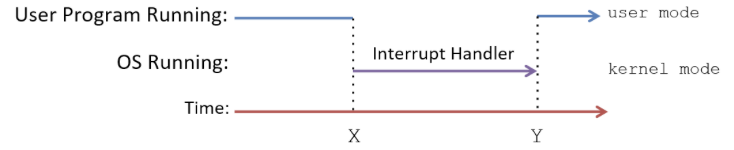
\includegraphics[scale=0.4]{img/interrupt.png}
        \caption{The CPU and interrupts. User code running on the CPU is interrupted (at time X on the time line), and OS interrupt handler code runs. After the OS is done handling the interrupt, user code execution is resumed (at time Y on the time line).} 
        \label{fig:interrupt}
      \end{figure}
    \end{definition}

    Now the question arises: how does the CPU know where to go when an system call or interrupt occurs? These are done through tables that map some unique ID number to some functionality. These tables are stored in a protected memory space reserved by the kernel. 

    \begin{definition}[System Call Table]
      This is done through the \textbf{system call table}, which is a table of addresses in memory that the CPU can jump to when a system call occurs. Each system call has a unique number $k$, and the handler function $k$ is called each time system call $k$ occurs. 
    \end{definition}

    \begin{example}[Common System Calls]
      Some common system calls, or \textbf{syscalls}, are shown below with their unique ID number (in Linux x64). 
      \begin{table}[H]
        \centering
        \caption{System Call Functions}
        \begin{tabular}{|c|l|l|}
        \hline
        \textbf{Number} & \textbf{Name} & \textbf{Description} \\ \hline
        0 & read & Read file \\ \hline
        1 & write & Write file \\ \hline
        2 & open & Open file \\ \hline
        3 & close & Close file \\ \hline
        4 & stat & Get info about file \\ \hline
        57 & fork & Create process \\ \hline
        59 & execve & Execute a program \\ \hline
        60 & \_exit & Terminate process \\ \hline
        62 & kill & Send signal to process \\ \hline
        \end{tabular}
      \end{table}
    \end{example}

    \begin{example}[Syscalls of Open] 
      Look at the following objdump file below. The corresponding C code just calls \texttt{open(filename, options)} and the corresponding syscall ID is \texttt{0x2}. We are simply loading the syscall ID into the \texttt{\%eax} register (only needs last 32 bits since the syscall IDs are quite small), which is then executed by the \texttt{syscall} instruction to go into the kernel mode. 
      \begin{lstlisting}
        00000000000e5d70 <__open>: 
        ...
        e5d79:  b8 02 00 00 00       mov    $0x2,%eax     # 2 is the open syscall number
        e5d7e:  0f 05                syscall              # return value in %rax
        e5d80:  48 3d 01 f0 ff ff   cmp    $0xfffffffffffff001,%rax 
        ... 
      \end{lstlisting}
      A negative number in \texttt{\%eax} gives an error corresponding to negative \texttt{errorno}. It is also worth mentioning that \texttt{\%eax} is used rather than \texttt{\%rdi} or \texttt{\%rsi} because we need these two parameter registers as arguments for the \texttt{open} function itself. 
    \end{example}

    Note that whether we are in the program stack or the kernel stack, we always have stack pointers and other registers to navigate them. In fact, for every CPU core, it has its own set of registers and its own kernel stack. 

    \begin{example}[Syscall of Read]
      If we have read syscall, then 
      \begin{enumerate}
        \item We use the syscall table to go to the trap handler for the read syscall. 
        \item The handler identifies the block and allocates a buffer. 
        \item Then it reads the block from the disk, which may take a while (in CPU time) since it is extremely slow for all IO tasks. The CPU, while waiting, can be put to sleep for other processes to run on the CPU. When the disk is done reading, it (the hardware) can send a hardware interrupt to the CPU, telling it that it is done. 
        \item Then it copies the block to the user buffer and returns from the syscall back into the user mode in the program state. 
      \end{enumerate}
    \end{example}

    \begin{definition}[Exception Table]
      This is done through the \textbf{exception table}, which is a table of addresses in memory that the CPU can jump to when an exception occurs. Each type of event has a unique exception number $k$, and the handler function $k$ is called each time exception $k$ occurs.\footnote{This is similar to a hardware implementation of a switch statement in C.}
      \begin{figure}[H]
        \centering 
        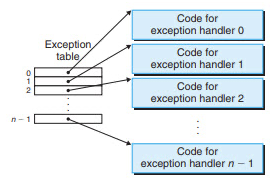
\includegraphics[scale=0.4]{img/exception_table.png}
        \caption{System call table is stored in a protected memory space reserved by the kernel.} 
        \label{fig:system_call_table}
      \end{figure}
    \end{definition}

    \begin{example}[Common Exception Numbers]
      Some common exception numbers are listed below. 
      \begin{table}[H]
        \centering
        \caption{Exception Summary}
        \begin{tabular}{|c|l|l|}
        \hline
        \textbf{Exception Number} & \textbf{Description} & \textbf{Exception Class} \\ \hline
        0 & Divide Error & Fault \\ \hline
        13 & General protection fault & Fault \\ \hline
        14 & Page fault & Fault \\ \hline
        18 & Machine check & Abort \\ \hline
        32-255 & OS-defined & Interrupt or trap \\ \hline
        \end{tabular}
      \end{table}
    \end{example}

    From the application's point of view, even if an interrupt happens, it just thinks it is running line by line. 

    \begin{definition}[Process Address Space]
      Interrupts can happen at any time, and one way to efficiently support this execution context switch from user mode to kernel mode is to do the following. At boot time, the OS loads its kernel code at a fixed location in RAM. Every time you create a new program state, the OS initializes a CPU register with the starting address of the OS handler function. On an interrupt, the CPU switches to kernel mode and executes OS interrupt handler code instructions that are accessible at the top addresses in every process’s address space. Because every process has the OS mapped to the same location at the top of its address space, the OS interrupt handler code is able to execute quickly in the context of any process that is running on the CPU when an interrupt occurs. This OS code can be accessed only in kernel mode, protecting the OS from user-mode accesses; during regular execution a process runs in user mode and cannot read or write to the OS addresses mapped into the top of its address space.\footnote{However, due to security reasons where the user space can read kernel space data, this is obsolete.}

      \begin{figure}[H]
        \centering 
        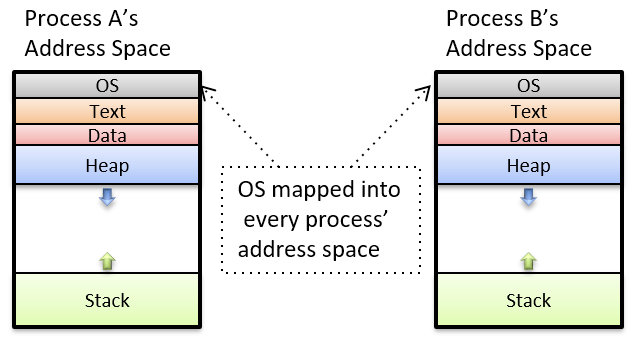
\includegraphics[scale=0.4]{img/process_address_space.png}
        \caption{Process address space: the OS kernel is mapped into the top of every process’s address space.} 
        \label{fig:process_address_space}
      \end{figure}
    \end{definition}

    In summary, a good visual is that each program runs as independent processes, with its own virtual address space (elaborated next) and the OS mediates access to shared resources.  

    \begin{figure}[H]
      \centering 
      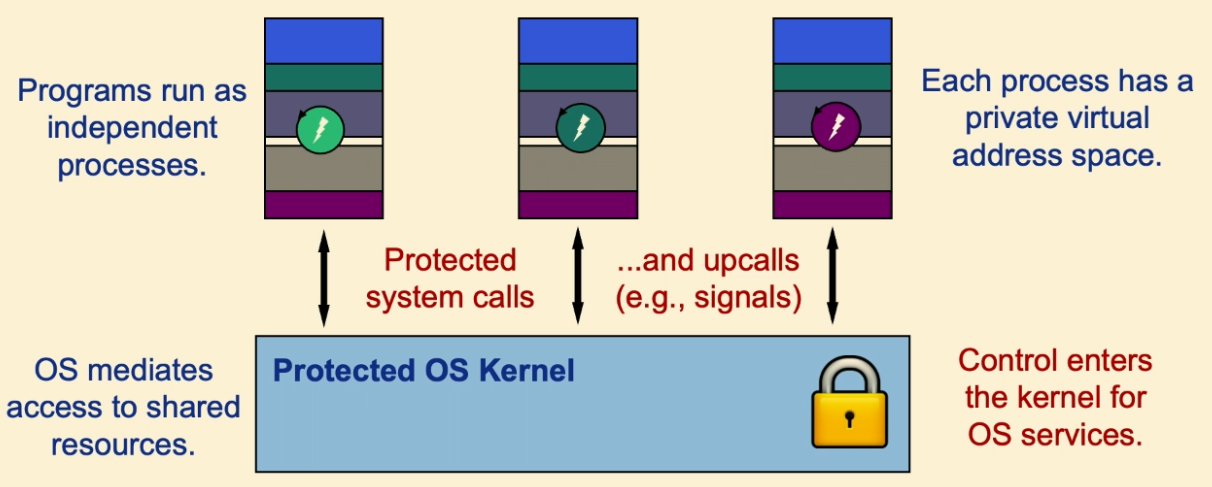
\includegraphics[scale=0.3]{img/os_multiple_programs.png}
      \caption{Multiple programs running and controlled by an operating system.} 
      \label{fig:os_multiple_programs}
    \end{figure}

    Each process can be in one of three states. It can either be currently running on the state, ready to run, or if there is a long IO operation, it can be blocked, which is then unblocked with a hardware interrupt. Usually anything that involves IO puts the state to blocked (e.g. reading data from disk, the keyboard, or the internet). The pool of processes that are concurrently running is the running and ready states. 
    \begin{figure}[H]
      \centering 
      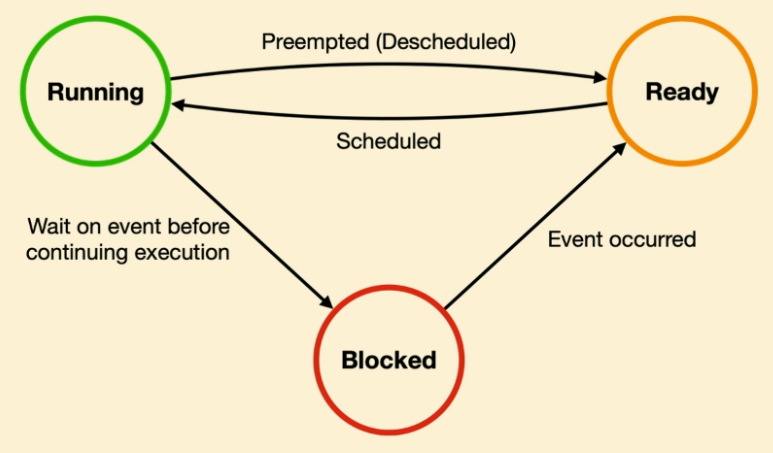
\includegraphics[scale=0.4]{img/3_process_states.png}
      \caption{Three states that a single process can be in. The pool of processes that are concurrently running is the running and ready states. The blocked state is waiting to be put back into this pool by a hardware interrupt.} 
      \label{fig:3_process_states}
    \end{figure}

    \begin{example}[Running a Binary]
      Therefore, to run a binary file \texttt{a.out}, 
      \begin{enumerate}
        \item The kernel first loads the binary file from disk into RAM.
        \item Then the OS kernel creates a new process with its own virtual memory stack and its global variables, etc. 
        \item Then the CPU's \texttt{\%rip} register point to the address of the \texttt{main} function. 
        \item The kernel's virtual memory space is mapped to the top of the process's virtual memory space, where it is not visible to the user mode. 
      \end{enumerate}
      \begin{figure}[H]
        \centering 
        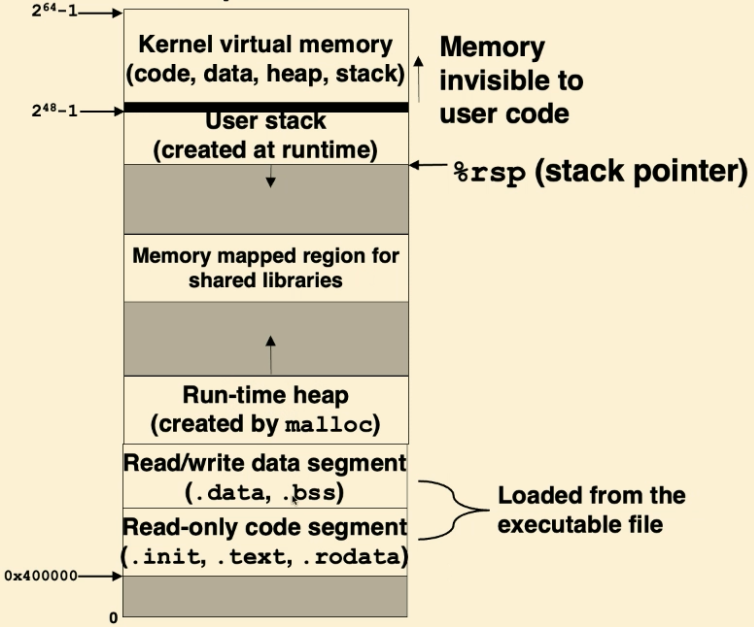
\includegraphics[scale=0.4]{img/process_space.png}
        \caption{The kernel's virtual memory space is mapped to the top of the process's virtual memory space.} 
        \label{fig:process_space}
      \end{figure}
    \end{example}

\section{Thread Management}

\section{Concurrency and Synchronization}

    So far, we've talked about everything as a sequential process of instructions. In practicality, we have improved this from the memory perspective by implementing caches, virtual memory, and swapping, but in the CPU perspective. In CPUs, we can't just simply increase the clock frequency indefinitely since there are physical limitations.\footnote{It turns out that power consumption increases faster than clock frequency, so it scales badly.} The current trend is to increase parallelism to compute faster, which is implemented with cores and threads. Let's clear some of these definitions up. 

    \begin{definition}[Processors, Cores]
      In almost every consumer computer, there exists one \textbf{processor} (CPU) in it. The CPU can have multiple \textbf{cores}. Each core has its own set of registers, L1/L2 cache, and possibly even a shared L3 cache. 
    \end{definition}

    Now these cores must run a certain program. Let's define what this means exactly. 

    \begin{definition}[Program, Process]
      A \textbf{program} can be thought of as a binary executable produced after linking. A \textbf{process} is a running instance of some program. 
      \begin{enumerate}
        \item It is identified by a \textbf{process ID (PID)} number. 
        \item It is run on a CPU core, with its own registers. 
        \item It has its own virtual address space, containing the code (instructions), heap, and pagetable that maps it to physical memory. 
      \end{enumerate}
    \end{definition}

    \begin{example}[Where to look for PIDs]
      We can see the PIDs either by using \texttt{htop} (for UNIX systems) or by looking at the \texttt{/proc} directory in Linux systems. Each directory name represents the PID of the process. 
      \begin{figure}[H]
        \centering
        \begin{subfigure}[b]{0.95\textwidth}
        \centering
          \begin{lstlisting}
            ubuntu@passionate-blesbok:/proc$ ls
            1     118   1368  26   44   590  762        cpuinfo      modules
            10    119   1369  27   448  599  763        crypto       mounts
            101   12    1370  28   45   6    764        devices      net
            1012  120   1371  29   46   605  765        diskstats    pagetypeinfo
            102   1232  138   3    467  608  769        driver       partitions
            103   1234  139   30   468  611  796        execdomains  pressure
            1031  1261  14    309  47   612  8          fb           sched_debug
            1037  129   15    31   471  613  801        filesystems  schedstat
            1038  13    16    32   473  629  810        fs           scsi
            104   132   17    33   474  638  822        interrupts   self
            1043  1342  18    34   475  651  836        iomem        slabinfo
            105   1353  180   35   48   666  850        ioports      softirqs
            106   1354  19    356  49   696  872        irq          stat
          \end{lstlisting}
          \caption{You can see the PIDs of the process by looking at the \texttt{/proc} directory. This changes quite often as processes are destroyed and created often, so to maybe track this in real time you might want to run \texttt{watch -n 0.1 'ls'}. }
          \label{fig:proc}
        \end{subfigure}

        \begin{subfigure}[b]{0.95\textwidth}
        \centering
          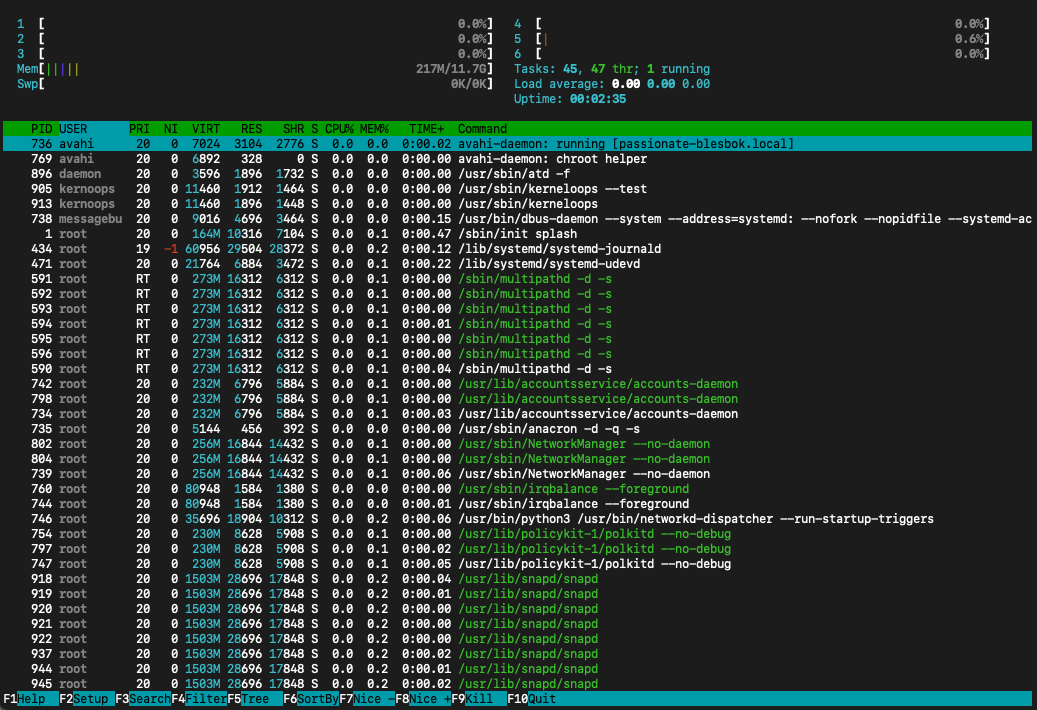
\includegraphics[width=\textwidth]{img/htop.png}
          \caption{You can see the PID number of each process (binary) running on the left column when running \texttt{htop} on UNIX systems. }
          \label{fig:htop}
        \end{subfigure}
        \caption{Two different ways to see the PIDs of all current processes. }
        \label{fig:}
      \end{figure}
      There is a specific numbering to each process. 
      \begin{enumerate}
        \item The process with PID 1 is always the kernel process. 
        \item The smaller PIDs (perhaps less than 300) are also reserved for the kernel, so don't kill it. 
      \end{enumerate}

      If you go into each process, you can see a few things.  
      
      \begin{figure}[H]
        \centering 
        \begin{lstlisting}
          ubuntu@passionate-blesbok:/proc/750$ sudo ls
          attr	    comm	     fd        map_files   net		  pagemap      sessionid     statm	    uid_map
          autogroup   coredump_filter  fdinfo    maps	   ns		  personality  setgroups     status	    wchan
          auxv	    cpuset	     gid_map   mem	   numa_maps	  projid_map   smaps	     syscall
          cgroup	    cwd		     io        mountinfo   oom_adj	  root	       smaps_rollup  task
          clear_refs  environ	     limits    mounts	   oom_score	  sched        stack	     timers
          cmdline     exe		     loginuid  mountstats  oom_score_adj  schedstat    stat	     timerslack_ns
        \end{lstlisting}
        \caption{There are many files in each PID folder that tells you about the process. } 
        \label{fig:pid_info}
      \end{figure}
      \begin{enumerate}
        \item To get information about the status of this process, you can \texttt{cat status}. 

        \item The virtual address space is stored in \texttt{pagemap}. If you're on an 64-bit machine, this file will be extremely big, so just \texttt{cat pagemap} won't work. Therefore you should try \texttt{cat maps}, which shows you something like the following. 

        \begin{lstlisting}
          ubuntu@passionate-blesbok:/proc/750$ sudo cat maps
          aaaac673c000-aaaac67e3000 r-xp 00000000 08:01 2576                       /usr/sbin/rsyslogd
          aaaac67f3000-aaaac67f6000 r--p 000a7000 08:01 2576                       /usr/sbin/rsyslogd
          aaaac67f6000-aaaac67fd000 rw-p 000aa000 08:01 2576                       /usr/sbin/rsyslogd
          aaaac67fd000-aaaac67fe000 rw-p 00000000 00:00 0 
          aaaadfe94000-aaaadfed7000 rw-p 00000000 00:00 0                          [heap] 
        \end{lstlisting}
        In here, you can see that the lefthand column represents the range of virtual memory address. The next column gives us the permissions (read, write, executable, shared/private). 
      \end{enumerate}
    \end{example}

  \subsection{Process Level Concurrency}

    \begin{definition}[Context Switch]
      Let us first start off with a single core system. At this point, everything is sequential, and to run all these processes at once\footnote{not programs, since there can be multiple instances of one program, like two Chrome instances. In fact, Chrome produces multiple processes to help run each part of the browser, so one program may translate to multiple processes. } we want to use system calls to transition between these processes. This is called a \textbf{context switch}. 

      \begin{figure}[H]
        \centering 
        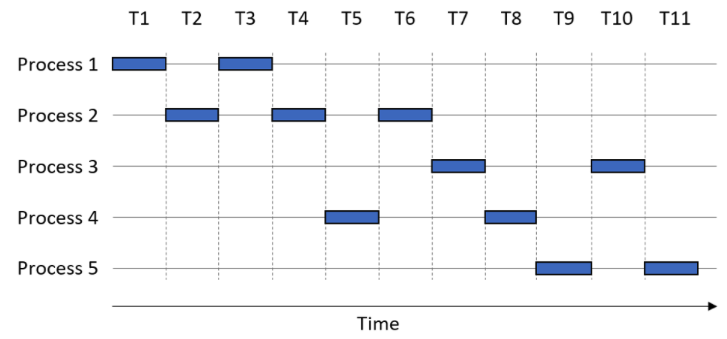
\includegraphics[scale=0.4]{img/seq_ex.png}
        \caption{5 processes may be executed as such on a single core. } 
        \label{fig:context_switch}
      \end{figure}
      Note that due to context switches, the \textbf{CPU time}, which is the time is takes to run a process on a CPU, is much shorter than the \textbf{wall-clock time}, which is the time a human perceives a process takes to complete. 
    \end{definition}

    Note that context switches are expensive. To do one, you must essentially replace two things. 
    \begin{enumerate}
      \item First, you need to clear out all the register values. This can be done by storing them in the current stack at the VAS, which then gets mapped through the page table into the physical address space. 
      \item Now the register values (like the instruction and stack pointers) are stored safely in the stack in the VAS, the actual page table must be swapped out too since each process must have its own virtual address space. 
    \end{enumerate}
    Since it is quite expensive to context switch all the time, the simplest thing to do is add more cores, which gives us the double benefit of distributing the process workload \textit{and} having to do less context switches. This is called \textbf{physical concurrency}, and given the same workload, it speeds up our computation absolutely. However, this can physically take us so far due to the limited number of cores, and we must go further and use \textbf{logical concurrency}. 

  \subsection{Thread Level Concurrency}

    It turns out that it is much more expensive to reload the page table of a new process rather than clearing out the register values. So, perhaps maybe we can try to implement multiple related ``processes'' that \textit{share} the same VAS, but have their own execution stream (i.e. own stack and registers). This is precisely the concept of a \textit{thread}. 

    \begin{definition}[Threads]
      \textbf{Threads} are multiple execution streams within a single process. To summarize them, a thread is an execution context within a process that has a... 
      \begin{enumerate}
        \item thread ID 
        \item its own stack frame 
        \item its own register context\footnote{This does not mean that each process has its own physical registers. It has its own \textit{value} that is loaded into the registers. The physical number of registers is determined by the number of CPU cores. }
      \end{enumerate}
      This is all that is really needed to execute some computation. Now, given that there are some number of threads in process $K$, they \textit{share} the same virtual address space (VAS), are all under the same PID, share the same code, static data, heap, and file table. The individual stacks living within the VAS are protected from each other to avoid stack overflow. 

      \begin{figure}[H]
        \centering 
        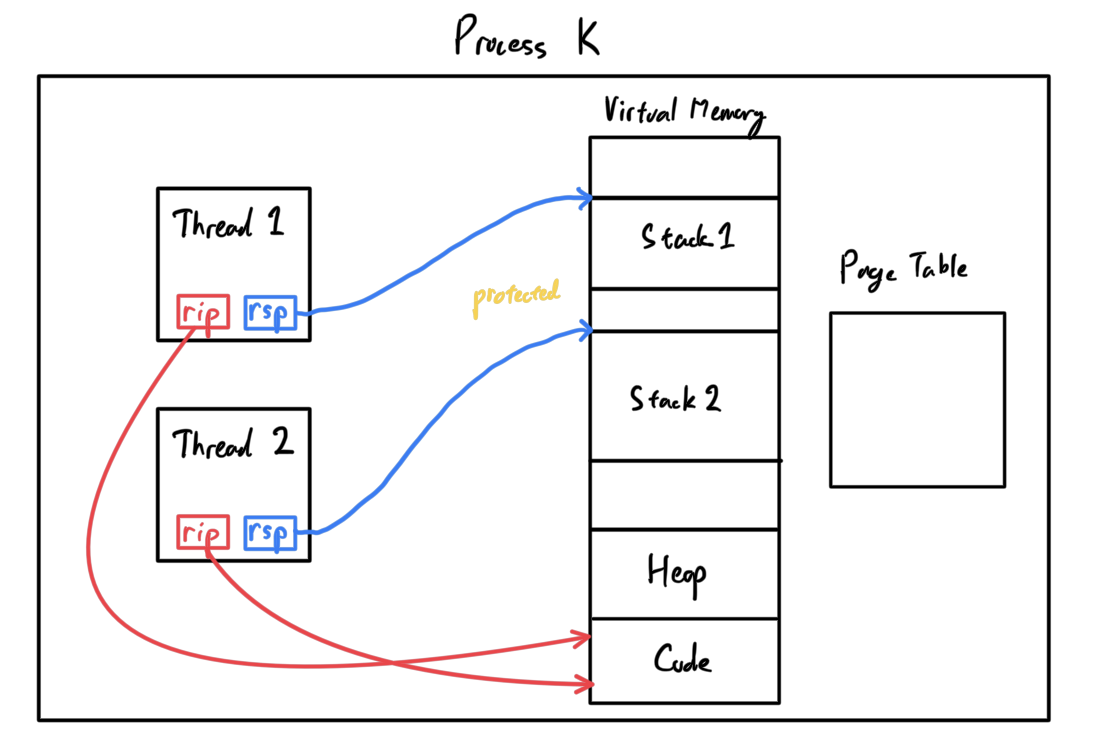
\includegraphics[scale=0.35]{img/2_threads.png}
        \caption{When there are two threads of a single process, the threads share the same virtual memory space. However, they each have their own set of registers. For example, they each have their own instruction pointer that points to the next line of code, along with their own stack pointer. Furthermore, to prevent stack overflow, there are protection mechanisms that prevent one stack from growing past a certain limit into another stack owned by a different thread. } 
        \label{fig:2_threads}
      \end{figure}
      Therefore, we can speed up our program in two ways. 
      \begin{enumerate}
        \item If we have one core, we can do context switching faster between each thread (since we only have to load the register values). 
        \item If we have multiple cores, we can take thread 1 and have it run on one core while taking thread 2 and running it on another core. This is really analogous to having two separate processes on two cores, but these two processes simply share the same VAS, with the same code, data, and heap. 
      \end{enumerate}
    \end{definition}

    Threads are advantageous for multiple reasons. First, by utilizing multiple cores we can speed up our program to reduce our \textit{CPU time}. However, if we are sharing threads between one core, we're not actually speeding up anything at all but rather reducing our \textit{wall-clock time}. The main speedup that we will feel is that latency heavy tasks will get offloaded to other threads, while more relevant programs can be run on the main thread. This is explained more in the following example. 

    \begin{example}[Mobile Application]
      If we have a single threaded messaging mobile app, then this is painfully slow since if we want to scroll down our messages while also sending and receiving messages, then we would have to wait for the message to receive from the server, into our disk, and into our memory, before the app responds when scrolling. 
      \begin{figure}[H]
        \centering 
        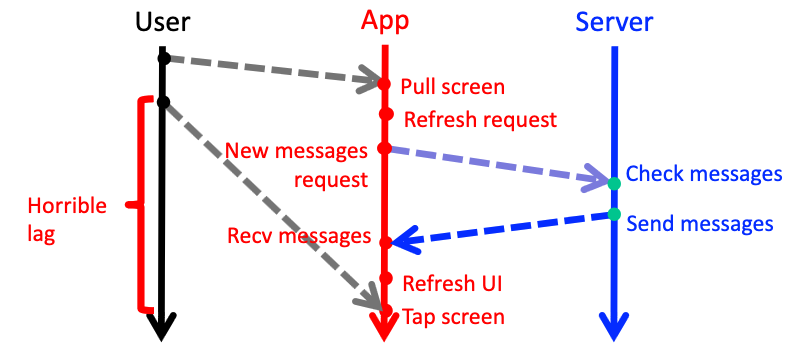
\includegraphics[scale=0.4]{img/single_threaded_app.png}
        \caption{Single threaded app.} 
        \label{fig:single_threaded_app}
      \end{figure}
      However, if we have a multithreaded app with one thread for the app UI and the other one for the server through a background thread, then we can have good UI response time. 
      \begin{figure}[H]
        \centering 
        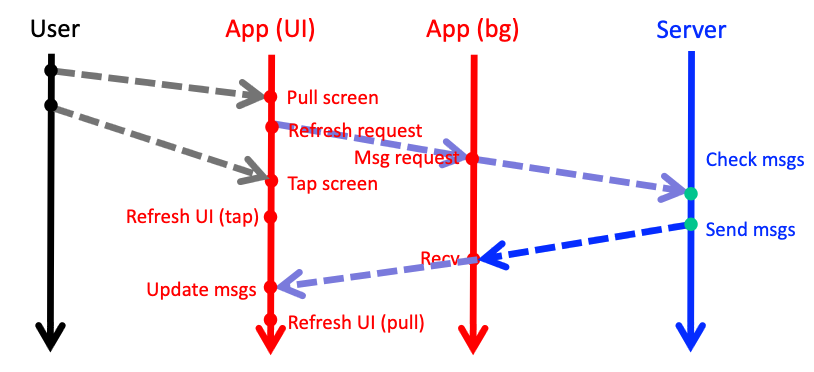
\includegraphics[scale=0.4]{img/multithreaded_app.png}
        \caption{Multithreaded app. Methods on the UI thread must be fast to ensure user satisfaction while anything slow can run on a background thread. } 
        \label{fig:multithreaded_app}
      \end{figure}
    \end{example}

    The following law gives us a certain bound on how much parallelization can help us. Note that this does not talk about the responsiveness of an application due to clever thread sharing. It just says given a certain amount of computational task, how much can we reduce the CPU time with parallelization? 

    \begin{theorem}[Amdahl's Law]
      Say that we have code that runs in 1 second. Given that proportion $f$ of our code can be parallelized, and the speedup for that portion is $N$, then the new time that our program will take is 
      \begin{equation}
        T_{\mathrm{new}} = (1 - f) + f/N
      \end{equation}
      since the sequential part $1 - f$ cannot be sped up, and the remaining parallel part $f$ can be sped up by distributing over $N$ cores. Therefore, defining the speedup as $T_{\mathrm{new}} / T_{\mathrm{old}}$, we get our total parallelized speedup is 
      \begin{equation}
        \frac{1}{(1 - f) + f/N}
      \end{equation}
      Note that it is bounded by the sequential portion as $N \rightarrow \infty$. 
      \begin{figure}[H]
        \centering 
        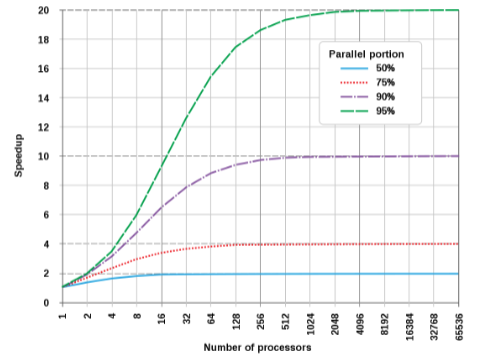
\includegraphics[scale=0.5]{img/amdahl.png}
        \caption{Amdahl's law for different $f$'s over multiple number of processors $N$.} 
        \label{fig:amdahl}
      \end{figure}
    \end{theorem}


    This is implemented in C with the \texttt{pthread.h} library, which is included in the standard library directory and follows the POSIX (Portable Operating System Interface) standard. Essentially, we want to do the following: 
    \begin{enumerate}
      \item Define a function that will be called for each thread. It must return a void pointer \texttt{void *} and its arguments must also be a void pointer \texttt{void *}. Think of this as our new main function for each stack that will be created from each thread.\footnote{Called a function pointer?} Since we are only restricted to a function taking in one void pointer argument, it is common to define a new struct like \texttt{arg\_t} that contains all the parameters you need to run each thread. The void pointer can be typecast into the struct pointer at the beginning of each thread function. 

      \item We create \texttt{pthread\_t} objects, which are the thread objects. 
      \item We call the \texttt{pthread\_create} function that takes in the pointer of the thread object, some settings, the function to be called, and its arguments. At this point, the operating system will determine how these threads will be run, so you can't make any sequential assumptions about them. 
      \item Then we join them using \texttt{pthread\_join}, which basically waits until all the threads are complete before \texttt{main} continues. 
    \end{enumerate}

    We will show two examples that go over this process. But more importantly, the concurrency of these two examples will show unpredictable behavior. 

    \begin{example}[Simply Print out Thread Number]
      We can make threads to print out the number. But these aren't really in the same order. 
      \begin{figure}[H]
        \centering 
        \noindent\begin{minipage}{.8\textwidth}
        \begin{lstlisting}[]{Code}
          #include <stdio.h> 
          #include <pthread.h>
          #include <stdlib.h>

          void* thread(void* args) {
            printf("Thread %d\n", *(int*)args); 
            return NULL; 
          }

          int main(int argc, char *argv[]) {
            int size = 10; 
            pthread_t threads[size]; 
            int rc, i;

            // thread creation 
            for (i = 0; i < size; i++) {
              rc = pthread_create(&threads[i], NULL, thread, &i); 
            }

            // join waits for the threads to finish 
            for (i = 0; i < size; i++) {
              rc = pthread_join(threads[i], NULL); 
            }
          return 0; 
          }
        \end{lstlisting}
        \end{minipage}
        \hfill
        \begin{minipage}{.19\textwidth}
        \begin{lstlisting}[]{Output}
          Thread 1
          Thread 2
          Thread 6
          Thread 3
          Thread 8
          Thread 5
          Thread 2
          Thread 4
          Thread 3
          Thread 3
          .
          .
          .
          .
          .
          .
          .
          .
          .
          .
          .
          .
          .
          .
          .
        \end{lstlisting}
        \end{minipage}
        \caption{Threads output shows that the order in which the functions are called cannot be predicted. } 
        \label{fig:threads}
      \end{figure}
    \end{example}

  \subsection{Atomicity Violation Bugs and Mutex Locks} 

    We see that there are some parts of the code that are not meant to be parallelized. 

    \begin{definition}[Atomicity-Violation Bugs] 
      This bug happens when the desired \textbf{atomicity} (indivisibility) among multiple memory accesses is violated. 
    \end{definition}

    \begin{example}[Atomicity-Violation in SQL]
      For example, if we have two threads doing the following (in MySQL): 
      \begin{lstlisting}
        Thread1:: 
        if (thd-> proc_info) {
          ...
          fputs(thd->proc_info); 
          ...
        }

        Thread2::
        thd->proc_info = NULL; 
      \end{lstlisting}
      If we pass the if statement but within it, \texttt{thd->proc\_info} becomes \texttt{NULL}, then this would be very bad. Therefore, we should put locks around. 
      \begin{lstlisting}
      pthread_mutex_t lock = PTHREAD_MUTEX_INITIALIZER; 

        Thread1:: 
        pthread_mutex_lock(&lock); 
        if (thd-> proc_info) {
          ...
          fputs(thd->proc_info); 
          ...
        }
        pthread_mutex_unlock(&lock); 

        Thread2::
        pthread_mutex_lock(&lock); 
        thd->proc_info = NULL; 
        pthread_mutex_unlock(&lock); 
      \end{lstlisting}
    \end{example}

    \begin{example}[Incrementing Shared Counter between Two Threads]
      The volatile keyword for \texttt{counter} means that it can be changed by all threads. 

      \begin{figure}[H]
        \centering 
        \noindent\begin{minipage}{.75\textwidth}
        \begin{lstlisting}[]{Code}
          #include <stdio.h> 
          #include <pthread.h>
          #include <stdlib.h>

          static volatile int counter = 0; 

          void* thread(void* args) {
            printf("%s : Start \n", (char*)args); 

            for (int i = 0; i < 10 * 1000 * 1000; i++) {
              counter += 1; 
            }

            printf("%s : End \n", (char*)args); 
            return NULL; 
          }

          int main(int argc, char *argv[]) {
            pthread_t thread1, thread2; 

            int rc; 
            rc = pthread_create(&thread1, NULL, thread, "A"); 
            rc = pthread_create(&thread2, NULL, thread, "B"); 

            rc = pthread_join(thread1, NULL); 
            rc = pthread_join(thread2, NULL); 

            printf("Counter : %d\n", counter); 
            return 0; 
          }
                      
        \end{lstlisting}
        \end{minipage}
        \hfill
        \begin{minipage}{.24\textwidth}
        \begin{lstlisting}[]{Output}
          A : Start 
          B : Start 
          A : End 
          B : End 
          Counter : 10229646
          .
          .
          A : Start 
          B : Start 
          B : End 
          A : End 
          Counter : 14965289
          .
          .
          A : Start 
          B : Start 
          A : End 
          B : End 
          Counter : 10086690
          .
          .
          .
          .
          .
          .
          .
          .
          .
          .
          .
        \end{lstlisting}
        \end{minipage}
        \caption{From looking at the behavior, we can see that the start and end times of thread A and thread B is complete unpredictable. It is only within the sequential nature within each thread (i.e. \texttt{X : start} must come before \texttt{X : End} that is predictable. More so, after all the increments, the total sum collected by counter isn't even 20 million!). The actual speed and ordering of this is determined at runtime. } 
        \label{fig:unpredictable}
      \end{figure}

      To really see what's going on here, we must look into the assmebly code behind this. If we focus on line 11 when the counter is incremented and look at its assembly, we see 
      \begin{lstlisting}
        7a7: 8b 05 0a 0b 20 00       mov    0x200b0a(%rip),%eax        # 200c1c <counter> 
        7ad: 83 c0 01                add    $0x1,%eax 
        7b0: 89 05 01 0b 20 00       mov    %eax,0x200b01(%rip)        # 200c1c <counter> 
      \end{lstlisting}
      What this means is that every thread consists of loading the \texttt{counter} value from the instruction pointer plus an offset into \texttt{\%eax}, then adding $1$ to it, and then storing it back to the same memory location (the rip changes, so the memory address between the 1st and 3rd line will be slightly different, but they are the same address). If we have threads $1$ and $2$, we can have the following possible interweavings: 
      \begin{enumerate}
        \item (1 loads, 1 adds, 1 stores, 2 loads, 2 adds, 2 stores). This would result in a $+2$. 
        \item (1 loads, 1 adds, 2 loads, 2 adds, 2 stores, 1 stores). This would result in a $+1$ since thread 2 loads before 1 could store the incremented version. 
        \item (1 loads, 2 loads, 1 adds, 2 adds, 1 stores, 2 stores). This would also result in a $+1$ for the same reasons as before. 
      \end{enumerate}
    \end{example}


    There is a big problem here: it seems that these things overwrite each other. 

    \begin{definition}[Data Race]
      We have just seen an example of a \textbf{data race}, which occurs if two or more threads concurrently accesses the same memory location with at least one write. The section of code where a data race can occur is called the \textbf{critical section}. 
    \end{definition}

    So how do we address this challenge of concurrency? This is where locks and mutexes come in. 

    \begin{definition}[Lock]
      A \textbf{lock} is a construct to enforce mutual exclusion in conflicting code sections (critical sections). It is implemented as a special data object in memory. We can use the API methods
      \begin{enumerate}
        \item \texttt{acquire()} or \texttt{lock()} is called when going into a critical section. 
        \item and \texttt{release()} or \texttt{unlock()} is called when going out of a critical section. 
      \end{enumerate}
      If the lock is already acquired by a thread and not released yet, then other threads will not be able to acquire the lock and execute the next instructions. There are two ways this is implemented. First, an incoming thread can wait if another thread holds the lock, called a \textbf{spinlock},\footnote{This is mainly implemented through kernel and used almost exclusively for OS development, not application development.} or it can be blocked, called a \textbf{mutex} (mutual exclusion).\footnote{This is mainly implemented in user space. }\footnote{This has a FIFO queue. }
    \end{definition}

    To implement this in C, there's a few things that we have to do. 
    \begin{enumerate}
      \item First, make a \texttt{pthread\_mutex\_t} global variable. 
      \item Then, make initialize the mutex before you create the threads and destroy the mutex after you join the threads in the \texttt{main} function. 
      \item Finally, put the specific locks and unlocks in the locations of the functions that the thread calls. 
    \end{enumerate}

    There are few strategies to correct the counter example above, which all produce the correct output \texttt{Counter: 20000000}. 
    \begin{enumerate}
      \item We can put the lock around the entire for loop of the \texttt{thread} function. However, this essentially takes us back to the sequential regime. 

      \begin{figure}[H]
        \centering 
        \begin{lstlisting}
          static volatile int counter = 0; 
          pthread_mutex_t mutex; // global declaration of mutex

          void* thread(void* args) {
            pthread_mutex_lock(&mutex); //acquire the mutex lock
            for (int i = 0; i < 10 * 1000 * 1000; i++) {
              counter += 1; 
            }
            pthread_mutex_unlock(&mutex); //release the mutex lock
            return NULL; 
          }

          int main(int argc, char *argv[]) {
            pthread_t thread1, thread2; 
            int rc; 
            rc = pthread_mutex_init(&mutex, NULL); //initialize the mutex
            rc = pthread_create(&thread1, NULL, thread, "A"); 
            rc = pthread_create(&thread2, NULL, thread, "B"); 
            rc = pthread_join(thread1, NULL); 
            rc = pthread_join(thread2, NULL); 
            pthread_mutex_destroy(&mutex); //destroy (free) the mutex
            printf("Counter : %d\n", counter); 
            return 0; 
          }
        \end{lstlisting}
        \caption{Putting the mutex locks around the entire for loop. } 
        \label{fig:first_try}
      \end{figure}

      \item A better idea to actually implement parallelization is to put the locks around the line that says \texttt{counter += 1;}. This is the critical code that loads the counter value from the stack into the register, increments it by $1$, and sends it back to the stack. We should isolate this so that no other threads can execute during these 3 assembly lines. 

      \begin{figure}[H]
        \centering 
        \begin{lstlisting}
          static volatile int counter = 0; 
          pthread_mutex_t mutex; // global declaration of mutex

          void* thread(void* args) {
            for (int i = 0; i < 10 * 1000 * 1000; i++) {
              pthread_mutex_lock(&mutex); //acquire the mutex lock
              counter += 1; 
              pthread_mutex_unlock(&mutex); //release the mutex lock
            }
            return NULL; 
          }

          int main(int argc, char *argv[]) {
            pthread_t thread1, thread2; 
            int rc; 
            rc = pthread_mutex_init(&mutex, NULL); //initialize the mutex
            rc = pthread_create(&thread1, NULL, thread, "A"); 
            rc = pthread_create(&thread2, NULL, thread, "B"); 
            rc = pthread_join(thread1, NULL); 
            rc = pthread_join(thread2, NULL); 
            pthread_mutex_destroy(&mutex); //destroy (free) the mutex
            printf("Counter : %d\n", counter); 
            return 0; 
          }
        \end{lstlisting}
        \caption{Now we put the locks within the counter. However, this is much slower since locking and unlocking are relatively expensive. It runs in 0.274s. } 
        \label{fig:second_try}
      \end{figure}

      \item The first two tries are not ideal, but what we can do is have each thread store its local work all within each of its stack, and then when it communicates with the shared memory on \texttt{counter}, this is where the locks should come in place. This has the double benefit of locking/unlocking very few times, along with protecting the critical section of the code. 

      \begin{figure}[H]
        \centering 
        \begin{lstlisting}
          static volatile int counter = 0; 
          pthread_mutex_t mutex; // global declaration of mutex

          void* thread(void* args) {
            int my_counter = 0; 
            for (int i = 0; i < 10 * 1000 * 1000; i++) {
              my_counter += 1; 
            }
            pthread_mutex_lock(&mutex); //acquire the mutex lock
            counter += my_counter; 
            pthread_mutex_unlock(&mutex); //release the mutex lock
            return NULL; 
          }

          int main(int argc, char *argv[]) {
            pthread_t thread1, thread2; 
            int rc; 
            rc = pthread_mutex_init(&mutex, NULL); //initialize the mutex
            rc = pthread_create(&thread1, NULL, thread, "A"); 
            rc = pthread_create(&thread2, NULL, thread, "B"); 
            rc = pthread_join(thread1, NULL); 
            rc = pthread_join(thread2, NULL); 
            pthread_mutex_destroy(&mutex); //destroy (free) the mutex
            printf("Counter : %d\n", counter); 
            return 0; 
          }
        \end{lstlisting}
        \caption{In here, we have each thread increment its own local version of the counter and store it in \texttt{my\_counter}. Then, we increment the global \texttt{counter} by the total \texttt{my\_counter}, which will require one mutex lock. It runs in 0.049s. }  
        \label{fig:third_try}
      \end{figure}
    \end{enumerate}

    \begin{example}[Inserting into Linked List]
      Inserting into a linked list is a sequential process, but what if we want to parallelize it with multiple threads? Consider the following code. 
      \begin{lstlisting}
        typedef struct __node_t {
          int key; 
          struct __node_t *next; 
        } node_t; 

        typedef struct __list_t {
          node_t *head; 
        } list_t; 

        void List_Init(list_t *L) {
          L -> head = NULL; 
        }

        void List_Insert(list_t *L, int key) {
          // insert a new node with the key value at the beginning of the list 
          node_t *new = malloc(sizeof(node_t)); 
          assert(new); 
          new -> key = key; 
          new -> next = L -> head; 
          L -> head = new; 
        }

        int main(void) {
          list_t L; 
          list_t *Lp = &L; 
          List_Init(Lp); 
          for (int i = 0; i < 10; i++) {
            List_Insert(Lp, i); 
          }
          return 0; 
        }
      \end{lstlisting}
      Say that we want to parallelize the creation of the length 10 linked list. Simply initializing some threads and calling \texttt{List\_Insert} 10 times won't properly create this linked list. This is because two threads may overwrite where \texttt{L -> head} points to. The most naive thing to do is to put locks around the whole function, but now we are back to the sequential regime! If we think about it, the \texttt{malloc} calls, asserting that there is viable memory, and assigning the input key value to \texttt{new -> key} does not overwrite anything else. It is only when we assign \texttt{new -> next} to the head value of \texttt{L} that things may get overwritten, so we put the locks shown below, while slightly modifying the \texttt{list} struct to have the \texttt{pthread\_mutex\_t} attribute. 
      \begin{lstlisting}
        typedef struct __list_t {
          node_t *head; 
          pthread_mutex_t lock; 
        } list_t; 

        void List_Init(list_t *L) {
          L -> head = NULL; 
          pthread_mutex_init(&L -> lock, NULL); 
        }

        void List_Insert(list_t *L, int key) {
          // insert a new node with the key value at the beginning of the list 
          node_t *new = malloc(sizeof(node_t)); 
          assert(new); 
          new -> key = key; 
          pthread_mutex_lock(&L->lock)
          new -> next = L -> head; 
          L -> head = new; 
          pthrea_mutex_unlock(&L->lock)
        }
      \end{lstlisting}
    \end{example}

  \subsection{Deadlock Bugs}

    Locks are extremely useful to segment out a portion of code that should be uninterrupted. However, there are many consequences of misusing it. 

    \begin{definition}[Deadlock Bugs]
      A \textbf{deadlock bug} happens when you make locks such that the program cannot run anymore. These aren't specific to threads, but also processes as well. They require the four preconditions: 
      \begin{enumerate}
        \item Mutual exclusion: you must have a lock to begin with to have a deadlock, so this is trivial. 
        \item Hold and Wait: Threads must have the ability to hold resources (e.g. the philosophers must hold forks which prevent others from taking them) . 
        \item No Preemption: Preemption refers to the ability to take the fork out of someone else's hand. So if you have a thread, you can first take lock A, then look at whether lock B is available. If not, then unlock A and try again. However, this can lead to a bunch of threads just simply picking up and putting down forks, causing a \textit{livelock}. 
        \item Circular Wait: That is, there exists a circular chain of threads such that each thread holds a resource needed by the next thread. A strategy is too define a fixed acquisition order for locks (e.g. lock A always before lock B). 
      \end{enumerate}
      You shouldn't try to hold multiple locks at once, but if you must, you should have a strategy to avoid deadlock. Choosing a lock order is the recommended way. 
    \end{definition}

    \begin{example}[Bank Accounts]
      Let's go through an example. Suppose we had the following code below. 
      \begin{lstlisting}
        struct account {
          pthread_mutex_t lock; 
          int balance; 
        }; 

        struct arg_t {
          struct account fromAcct; 
          struct account toAcct; 
          int amt; 
        }; 

        pthread_mutex_t mutex; // global declaration of mutex

        void* Transfer(void* args) {

          struct arg_t* data = (struct arg_t*)args; 

          struct account* fromAcct = &(data -> fromAcct); 
          struct account* toAcct = &(data -> toAcct); 
          int amt = data -> amt; 


          pthread_mutex_lock(&fromAcct->lock);
          pthread_mutex_lock(&toAcct->lock);

          fromAcct->balance -= amt;
          toAcct->balance += amt;

          pthread_mutex_unlock(&fromAcct->lock);
          pthread_mutex_unlock(&toAcct->lock);

          return NULL; 
        }
      \end{lstlisting}
      Suppose that Threads 0 and 1 are executing concurrently and represent users A and B, respectively. Now consider the situation in which A and B want to transfer money to each other: A wants to transfer 20 dollars to B, while B wants to transfer 40 to A.

      Both threads concurrently execute the \texttt{Transfer} function. Thread 0 acquires the lock of acctA while Thread 1 acquires the lock of acctB. Now consider what happens. To continue executing, Thread 0 needs to acquire the lock on acctB, which Thread 1 holds. Likewise, Thread 1 needs to acquire the lock on acctA to continue executing, which Thread 0 holds. Since both threads are blocked on each other, they are in deadlock.

      This can be simply fixed by rearranging the locks so that each lock/unlock pair surrounds only the balance update statement associated with it. 
      \begin{lstlisting}
      void *Transfer(void *args){
        //argument passing removed to increase readability
        //...

        pthread_mutex_lock(&fromAcct->lock);
        fromAcct->balance -= amt;
        pthread_mutex_unlock(&fromAcct->lock);

        pthread_mutex_lock(&toAcct->lock);
        toAcct->balance += amt;
        pthread_mutex_unlock(&toAcct->lock);

        return NULL;
      } 
      \end{lstlisting}
    \end{example}

    \begin{example}[Dining Philosopher's Problem]
      There are 5 philosophers at a roundtable with 5 plates of food with 5 forks. Each philosopher needs two forks (both on their left and on their right) to start eating their plate. However, there can be a deadlock if every philosopher takes the fork on their right and is always waiting for the left fork (this happens due to a circular dependency). 
      \begin{enumerate}
        \item One way to resolve this issue is to set an ID to every fork and have the philosophers always take the lower ID fork first before trying to take the higher ID. Then this resolves and at least one philosopher can eat. 
      \end{enumerate}
    \end{example}

    \begin{example}[Set-Intersection Problem]
      Again, like the bank account section, we have the following code that can create deadlocks if there is a code that attempts to compute $A \cap B$ and $B \cap A$ at similar times. 
      \begin{lstlisting}
        set_t *set_intersection(set_t *s1, set_t *s2) {
          set_t *result = set_create(); 
          pthread_mutex_lock(&s1->lock); 
          pthread_mutex_lock(&s2->lock); 

          for (int i = 0; i < s1->size; i++) {
            if (set_contains(s2, s1->data[i])) {
              set_add(result, s1->data[i]); 
            }
          }

          pthread_mutex_unlock(&s2->lock); 
          pthread_mutex_unlock(&s1->lock); 
          return result; 
        }
      \end{lstlisting}
      Like using the IDs and ordering, we can resolve this by grabbing locks in a defined order, say from high to low. Therefore, we replace the locks as such.
      \begin{lstlisting}
        if (&m1 > &m2) {
          pthread_mutex_lock(&m1); 
          pthread_mutex_lock(&m2); 
        } else {
          pthread_mutex_lock(&m2); 
          pthread_mutex_lock(&m1); 
        }
      \end{lstlisting}
      However, this still creates a deadlock if we compute $A \cap A$, so we should place a deadlock. 
    \end{example}

    It turns out that we can make logically equivalent code without locks! By using atomic primitives that have implementations in C, we can create wait-free algorithms. For example, consider the \texttt{int CompAndSwap(int* addr, int expected, int new)} function. If \texttt{*addr == expected}, then we set \texttt{*addr} to \texttt{new} and return $1$. Otherwise, we do nothing and return $0$. Then, the two pieces of code are equivalent, but the advantage of the RHS is that there is never a deadlock. \begin{enumerate}
      \item In the left, we pass by pointer to increment a variable. 
      \item In the right, we first set \texttt{old} to the value of \texttt{val}, and if the value of \texttt{val} is equal to \texttt{old} (which may not always be true if some other thread modifies this value), then we set \texttt{old = *val} again and increment it by \texttt{amt}. 
    \end{enumerate}
    \noindent\begin{minipage}{.5\textwidth}
    \begin{lstlisting}[]{Code}
      void add(int *val, int amt) {
        pthread_mutex_lock(&m); 
        *val += amt; 
        pthread_mutex_unlock(&m); 
      }
      .
    \end{lstlisting}
    \end{minipage}
    \hfill
    \begin{minipage}{.49\textwidth}
    \begin{lstlisting}[]{Output}
      void add(int *val, int amt) {
        do {
          int old = *val;    
        }
        while(!CompAndSwap(val, old, old+amt)); 
      }
    \end{lstlisting}
    \end{minipage}
    However, the left hand, despite the risk of deadlocks, is still recommended. The mutex API allows for better distribution of CPU. 

       
  \subsection{Order Violation Bugs and Condition Variables} 

    \begin{definition}[Order Violation Bugs]
      An \textbf{order violation bug} happens when the desired order between two memory accesses is flipped, i.e. A should always be executed before B, but the order is not enforced during execution. 
      \begin{enumerate}
        \item For example, one thread that acts on a linked list may already assume that the linked list is initialized when it is not. Therefore, we should have these threads wait until initialization. 
        \item Another example is if there is a set of producers and consumers that manage the flow of items through a buffer. If there is no good, then consumers cannot consume and they must wait. If the supply is full then the producers must wait. This also requires some process of waiting. 
      \end{enumerate}
    \end{definition}

    We can use a regular conditional to check, but this may not be efficient due to the following example. 

    \begin{example}[Condition Checks with Vanilla While Loops]
      Say that you want to call the following function on a linked list, but you must wait until the list is not \texttt{NULL}. 
      \begin{lstlisting}
        int getItem(list_t *list) {
          pthread_mutex_lock(&list -> m); 
          // TODO: wait until list is non-empty
          int item = list -> head -> item; 
          list -> head = list -> head -> next; 
          pthread_mutex_unlock(&list -> m);  
          return item; 
        }
      \end{lstlisting}

      To check whether \texttt{list} is not a null pointer, we can simply use a while loop to check. 

      \begin{figure}[H]
        \centering 
        \noindent\begin{minipage}{.5\textwidth}
        \begin{lstlisting}[]{Code}
          int tryGetItem(list_t *list, int *out) {
            int success = 0; 
            ptherad_mutex_lock(&list -> m); 
            if (list -> head) {
              success = 1; 
              *out = list -> head -> item;
              list -> head = list -> head -> next; 
            }
            pthread_mutex_unlock(&list -> m); 
            return success; 
          }
          .
          .
        \end{lstlisting}
        \end{minipage}
        \hfill
        \begin{minipage}{.49\textwidth}
        \begin{lstlisting}[]{Output}
          int getItem( list_t *list) {
            pthread_mutex_lock(&list -> m); 
            // TODO: wait until list is non-empty 
            while (list -> head == NULL) {
              pthread_mutex_unlock(&list -> m); 
              yield();        // optional 
              pthread_mutex_lock(&list -> m); 
            }
            int item = list -> head -> item; 
            list -> head = list -> head -> next; 
            pthread_mutex_unlock(&list -> m);  
            return item; 
          }
        \end{lstlisting}
        \end{minipage}
        \caption{On the LHS, this returns $0$ if the retrieval is not successful, and so you must wrap this function within some while loop to check if it is actually successful. On the RHS, we can use the \texttt{yield()} function which gives control to the OS to schedule another thread. }
        \label{fig:cpu_waste}
      \end{figure}

      This constant checking through a while loop leads to a waste of CPU resources. Therefore, we want to put the thread to sleep while there is no element in \texttt{list} so other processes can use the CPU core. This is the motivation behind \textit{conditional variables}. 
    \end{example}

    \begin{definition}[Condition Variables]
      \textbf{Condition Variables} force a thread to be blocked until a particular condition is reached. This construct is useful for scenarios in which a condition must be met before the thread does some work.
      \begin{enumerate}
        \item Every CV is bound to exactly one mutex. This is because the state of a condition, even if true on one thread, can be changed immediately by another thread, so some sort of locking is needed. 
        \item Condition variables have the type \texttt{pthread\_cond\_t}. 
        \item To initialize a condition variable, use the \texttt{pthread\_cond\_init} function. 
        \item To destroy it, use \texttt{pthread\_cond\_destroy}. 
        \item \texttt{pthread\_cond\_wait(\&cond, \&mutex)} takes the address of a condition variable \texttt{cond} and a mutex \texttt{mutex} as its arguments. It causes the calling thread to block on the condition variable cond until another thread signals it (or "wakes" it up).
        \item The \texttt{pthread\_cond\_signal(\&cond)} function causes the calling thread to unblock (or signal) another thread that is waiting on the condition variable \texttt{cond} (based on scheduling priority). If no threads are currently blocked on the condition, then the function has no effect. Unlike \texttt{pthread\_cond\_wait}, the \texttt{pthread\_cond\_signal} function can be called by a thread regardless of whether or not it owns the mutex in which \texttt{pthread\_cond\_wait} is called.
      \end{enumerate}
    \end{definition}

    It is important to know about the states that a thread can be in. It can either be currently running/active, ready to run (perhaps through a syscall), or blocked. 
    \begin{figure}[H]
      \centering 
      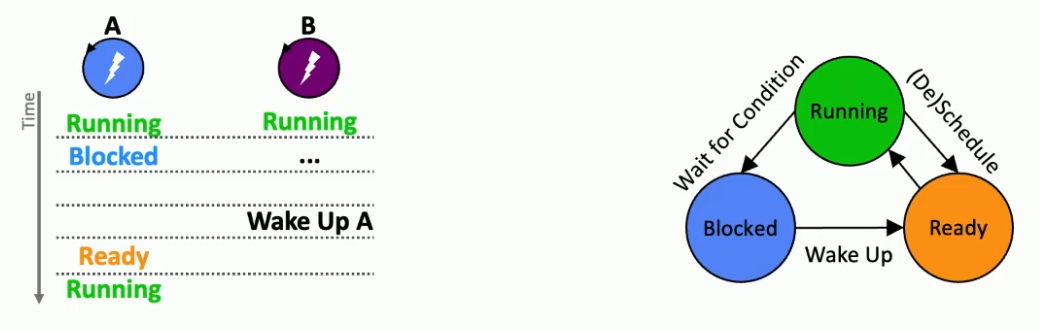
\includegraphics[scale=0.4]{img/states.png}
      \caption{Note that the only way a thread can be blocked is if it is waiting for a condition to happen. If that condition happened and a signal arrives at the thread, then it ``wakes up.'' Condition variables allow these thread to go in and out of the blocked state.} 
      \label{fig:states}
    \end{figure}

    With this, the general design pattern is as such. 

    \begin{theorem}[Condition Variable Design Pattern]
      To implement this effectively, we must first identify a state that will be accessed by 2+ threads concurrently and add locks to protect the shared state. If we need to wait on some condition, we use condition variables.  

      \noindent\begin{minipage}{.5\textwidth}
      \begin{lstlisting}[]{Code}
        methodThatWaits() {
          pthread_mutex_lock(&m); 

          // Read/write shared state 

          while (!checkSharedState()) {
            pthread_cond_wait(&cv, &m); 
          }

          // Read/write shared state 

          pthread_mutex_unlock(&m); 
        }
      \end{lstlisting}
      \end{minipage}
      \hfill
      \begin{minipage}{.49\textwidth}
      \begin{lstlisting}[]{Output}
        methodThatSignals() {
          ptherad_mutex_lock(&m); 

          // Read/write shared state 

          // If checkSharedState() is now true 
          pthread_cond_signal(&cv); 

          // Read/write shared state 

          pthread_mutex_unlock(&m); 
        }
        .
      \end{lstlisting}
      \end{minipage}
    \end{theorem}

    The implementation is quite complex at first, so let's go through an example. 

    \begin{example}[Soda Machine]
      Say that we want to model a soda machine, with consumers taking soda from the machine and producers filling the machine up. 
      \begin{enumerate}
        \item We'd like to create some variables that encode the state of the soda machine. This is the \textbf{shared state}. 
          \begin{lstlisting}
            static volatile int numSodas; 
            #define MaxSodas 100; 
          \end{lstlisting}

        \item We also want to implement \textit{one} lock to protect all shared states, say 
          \begin{lstlisting}
            pthread_mutex_t sodaLock; 
          \end{lstlisting}
          This allows us to implement mutual exclusion so that only one thread can manipulate the machine (state) at a time. 

        \item The \textbf{ordering constraints} are that the consumer must wait if the machine is empty (CV \texttt{hasSoda}), and the producer must wait if the machine is full (CV \texttt{hasRoom}). 

        \item The first thing we must do is make sure that the consumer and producer function has a lock and unlock over its body since both functions modify the vending machine. 

          \noindent\begin{minipage}{.5\linewidth}
          \begin{lstlisting}[]{Code}
            consumer() {
              pthread_mutex_lock(&sodaLock); 

              // take a soda from machine

              pthread_mutex_unlock(&sodaLock); 
            }
          \end{lstlisting}
          \end{minipage}
          \hfill
          \begin{minipage}{.49\linewidth}
          \begin{lstlisting}[]{Output}
            producer() {
              pthread_mutex_lock(&sodaLock); 

              // add a soda to machine

              pthread_mutex_unlock(&sodaLock); 
            }
          \end{lstlisting}
          \end{minipage}

        \item Moreover, the consumer and producer's actions of taking or adding soda is dependent on the state already. For the consumer, it should \textbf{wait} if the machine is empty for a signal that notifiies that it is not empty. Once the consumer receives the signal, it takes a soda and can send a signal that the machine is not full to the producer function. 

          \noindent\begin{minipage}{.5\linewidth}
          \begin{lstlisting}[]{Code}
            consumer() {
              pthread_mutex_lock(&sodaLock); 
              // wait if empty
              // take a soda from machine
              // notify that it is not full 
              pthread_mutex_unlock(&sodaLock); 
            }
          \end{lstlisting}
          \end{minipage}
          \hfill
          \begin{minipage}{.49\linewidth}
          \begin{lstlisting}[]{Output}
            producer() {
              pthread_mutex_lock(&sodaLock); 
              // wait if full 
              // add a soda to machine
              // notify that it is not empty 
              pthread_mutex_unlock(&sodaLock); 
            }
          \end{lstlisting}
          \end{minipage}

        \item To put this into code, we finally have 

          \noindent\begin{minipage}{.5\linewidth}
          \begin{lstlisting}[]{Code}
            consumer() {
              pthread_mutex_lock(&sodaLock); 

              while (numSodas == 0) {   
                // while empty 
                wait(sodaLock, hasSoda); 
              }
              numSodas -= 1;    // take soda 
              signal(hasRoom); 
              pthread_mutex_unlock(&sodaLock); 
            }
          \end{lstlisting}
          \end{minipage}
          \hfill
          \begin{minipage}{.49\linewidth}
          \begin{lstlisting}[]{Output}
            producer() {
              pthread_mutex_lock(&sodaLock); 

              while (numSodas == MaxSodas) {
                wait(sodaLock, hasRoom); 
              }

              numSodas += 1;    // add soda 
              signal(hasSoda);  
              pthread_mutex_unlock(&sodaLock); 
            }
          \end{lstlisting}
          \end{minipage}
      \end{enumerate}
      Let's go through this. From the consumer function, we have: 
      
      \begin{enumerate}
        \item The consumer function can start by first acquiring a lock on the \texttt{sodaLock} mutex using \texttt{pthread\_mutex\_lock()}. This ensures that only one consumer thread can access the shared resources (e.g., \texttt{numSodas}) at a time.

        \item It then enters a while loop\footnote{We want this to be a while loop since we want to reevaluate the condition even after reacquiring the lock. } that checks if \texttt{numSodas} is zero. If \texttt{numSodas} is zero, it means there are no sodas available for consumption. In this case, the consumer thread calls the \texttt{wait()} function, which unlocks the \texttt{sodaLock} mutex and waits for a signal on the \texttt{hasSoda} condition variable. This allows other threads to acquire the lock and proceed.

        \item When the consumer thread receives a signal indicating that sodas are available (\texttt{hasSoda} condition variable), it wakes up and reacquires the lock on \texttt{sodaLock}.

        \item The consumer thread then decrements \texttt{numSodas} by 1, indicating the consumption of a soda.

        \item After consuming a soda, the consumer thread signals the \texttt{hasRoom} condition variable using the \texttt{signal()} function. This notifies any waiting producer threads that there is now room available in the soda buffer.

        \item Finally, the consumer thread unlocks the \texttt{sodaLock} mutex using \texttt{pthread\_mutex\_unlock()}, allowing other threads to access the shared resources.
      \end{enumerate}
      
      From the producer function, we have: 

      \begin{enumerate}
        \item The producer function can start by first acquiring a lock on the \texttt{sodaLock} mutex using \texttt{pthread\_mutex\_lock()}. This ensures that only one producer thread can access the shared resources at a time.

        \item It then enters a while loop that checks if \texttt{numSodas} is equal to \texttt{MaxSodas}. If \texttt{numSodas} is equal to \texttt{MaxSodas}, it means the soda buffer is full, and the producer cannot add more sodas. In this case, the producer thread calls the \texttt{wait()} function, which unlocks the \texttt{sodaLock} mutex and waits for a signal on the \texttt{hasRoom} condition variable. This allows other threads to acquire the lock and proceed.

        \item When the producer thread receives a signal indicating that there is room available in the soda buffer (\texttt{hasRoom} condition variable), it wakes up and reacquires the lock on \texttt{sodaLock}.

        \item The producer thread then increments \texttt{numSodas} by 1, indicating the production of a new soda.

        \item After producing a soda, the producer thread signals the \texttt{hasSoda} condition variable using the \texttt{signal()} function. This notifies any waiting consumer threads that a soda is now available for consumption.

        \item Finally, the producer thread unlocks the \texttt{sodaLock} mutex using \texttt{pthread\_mutex\_unlock()}, allowing other threads to access the shared resources.

      \end{enumerate}
      Note that we must have a while loop since if the producer ended up broadcasting the \texttt{hasSoda} condition to say 10 threads when there are 5 sodas, then 5 of those threads will get a soda while 5 may not, and this possibility should be detected by the while loop. 
    \end{example}

\section{Memory Management}

  \subsection{Virtual Memory}

    We have mentioned that there is a problem where two different application developers, who have linked their own C files to create binaries, can be installed on one computer and run at the same time. However, the linking has already been finished and the memory addresses of the symbols in each executable are fixed. This can be a problem if there are overlaps in the memory addresses. 

    \begin{definition}[Virtual Memory]
      The actual main memory of our system is referred to as the \textbf{physical memory}. To prevent such overlaps, the kernel and each user process has its own \textbf{virtual memory}. That is, there exists a \textbf{memory management unit (MMU)} in the CPU that translates virtual addresses to physical addresses through a hashmap. 
      \begin{figure}[H]
        \centering 
        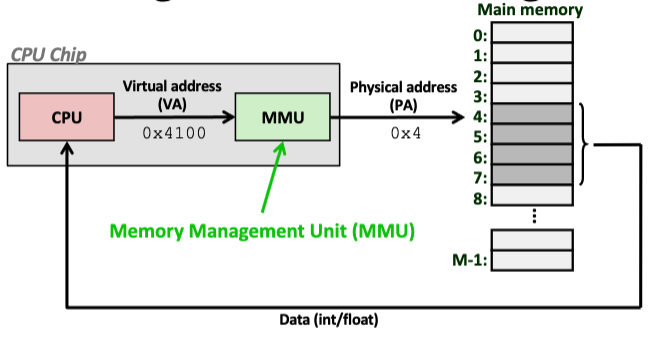
\includegraphics[scale=0.4]{img/mmu.png}
        \caption{Memory management unit maps each virtual address to a physical address.} 
        \label{fig:mmu}
      \end{figure}
      This allows the kernel to map the virtual memory of each process to the physical memory.
      \begin{figure}[H]
        \centering 
        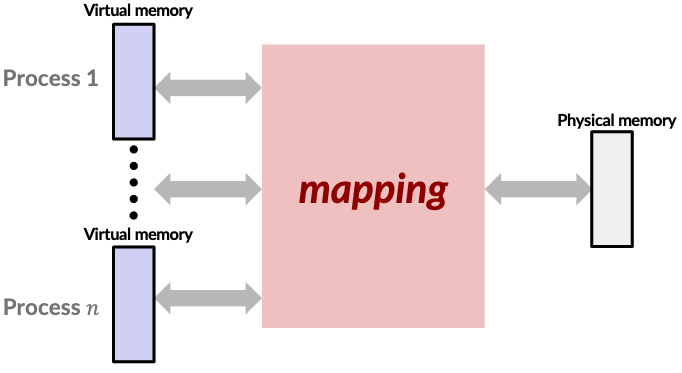
\includegraphics[scale=0.4]{img/vm_map.png}
        \caption{Each process has its own virtual memory space, which is mapped by the MMU to the physical memory space. } 
        \label{fig:vm_map}
      \end{figure}
    \end{definition}

    \begin{example}[Virtual and Physical Memory Size]
      Given a $n$-bit machine with $2^m$-bytes of memory, $n > m$ and so there are more virtual addresses than physical addresses. If we have a 64-bit machine with 16GB of memory, then there are $2^{64}$ virtual addresses and $2^{3} \cdot 2^{34} = 2^{37}$ bits of physical memory. If there are 8 processes running then there are $8 \cdot 2^{64} = 2^{67}$ bits of virtual memory. 
    \end{example}

    There are many properties of virtual memory that solves a lot of problems and makes things more convenient. The main property is called \textbf{indirection} which means that the virtual memory is not the actual physical memory. 
    \begin{enumerate}
      \item The first problem is that there are much more virtual addresses than physical addresses. Even storing a table for one process would take up more than all of your RAM. Therefore, for every byte in main memory, there exists one physical address (PA) and zero, one, or more virtual addresses (VA). We will elaborate on the specifics of this implementation later. 
      \item We also need to have memory management. Every process has its own stack, heap, \texttt{.text}, and \texttt{.data} sections. We must be able to allocate and deallocate memory and fit this accordingly. 
      \item We also need to have protection. We need to ensure that one process cannot read or write to another process's memory.
      \item While we want isolation, we also want sharing between processes if needed (e.g. signing into Slack using Google on a browser). Furthermore, if there are multiple calls of the \texttt{printf} function, we can just have a single copy of the \texttt{printf} function in memory rather than having multiple copies for each process. This can be done through the concept of permissions. 
    \end{enumerate}

    Let's talk about how we should actually map these addresses. One property of this mapping is that we want contiguous addresses both in the virtual and the physical level so that we can store arrays, exploit locality, etc. Therefore, we can use larger blocks known as \textit{pages}. Just like how we have divided memory addresses into sections that can be used to map to caches, we can divide the memory addresses into sections that can be used to map to the physical memory. Note that this also takes care of the first problem partially since now we can fit this table in the memory. 
      
    \begin{definition}[Page]
      Both in virtual and physical memory, an $n$-bit address can be divided into a \textbf{page number} and an \textbf{offset}. The page number is $n - 12$ and the offset is $12$ bits. The page number is used to index into a \textbf{page table} that maps the page number to a physical address. 
      \begin{figure}[H]
        \centering 
        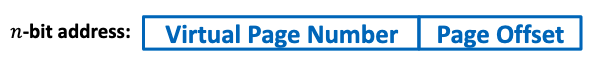
\includegraphics[scale=0.4]{img/page.png}
        \caption{A page is a contiguous block of memory addresses.} 
        \label{fig:page}
      \end{figure}
      While the entire page table is stored in memory (at memory stored by a protected CPU register), a portion of the page table is stored in the CPU cache. 
      \begin{enumerate}
        \item The virtual page number (VPN) is equivalent to the block number. 
        \item The page offset is equivalent to the block offset. 
      \end{enumerate}
    \end{definition}

    \begin{example}[Page Number]
      In a 64-bit machine with 16GB of RAM, you have $2^{64} / 2^{12} = 2^{52}$ virtual pages and $2^{37} / 2^{12} = 2^{25}$ physical pages. 
    \end{example}

    Therefore, our translation table is really a map from a virtual page number to a physical page number, rather than a virtual address to a physical address. This is created at runtime. Therefore, 
    \begin{enumerate}
      \item The virtual page number $VP$ is mapped through some map $M$ to get the physical page number $PP$. 
      \item The virtual offset is the same as the physical offset. 
    \end{enumerate}

    \begin{definition}[Page Table]
      The \textbf{page table} is a hashmap that maps the virtual page number to the physical page number defined as the mapping 
      \begin{equation}
        H: \underbrace{(VP,m)}_{\text{64 bits}} \longrightarrow PP
      \end{equation}
      Each input-output pair is called a \textbf{page table entry (PTE)}, and virtual memory is \textbf{fully associative}, meaning that any virtual page can be placed in any physical page, though it requires a large mapping function (the PT), which is different from CPU caches. 
      \begin{figure}[H]
        \centering 
        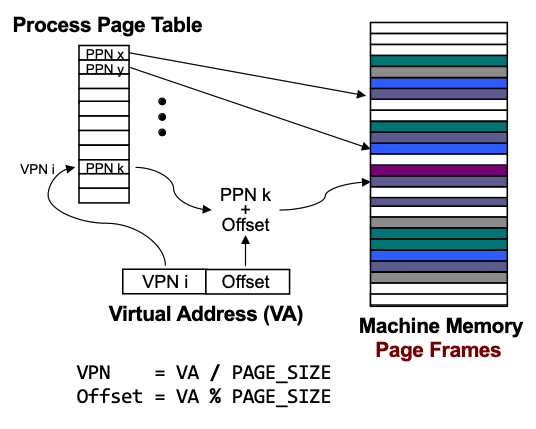
\includegraphics[scale=0.4]{img/page_table.png}
        \caption{The page table only needs the virtual page number plus the metadata to map to the physical page number. The offset is provided by the virtual memory address itself. } 
        \label{fig:page_table}
      \end{figure}
      Note that while we want to store the 52-bit VP in the page table, the actual input is still 64-bits, with 12 bits of metadata $m$. This metadata contains some information about the following 
      \begin{enumerate}
        \item A bit that indicates whether the page is a read, write, or executable piece of code (3 bits). 
        \item A bit that indicates whether the page is valid or not. 
      \end{enumerate}
      \begin{figure}[H]
        \centering 
        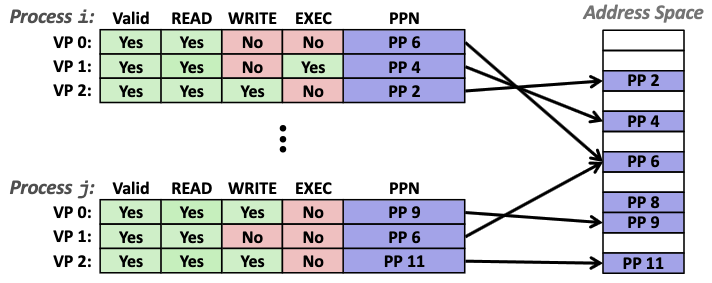
\includegraphics[scale=0.4]{img/permissions_vm.png}
        \caption{The page table entry contains the physical page number and some metadata.} 
        \label{fig:permissions_vm}
      \end{figure}
    \end{definition}

    Therefore, if you malloc, you are really just allocating some virtual memory addresses, which then get mapped to physical memory addresses in one or more pages. 

    \begin{definition}[Page Fault]
      It is clear that not every virtual page number can be mapped to a physical page number. If it turns out that a \textbf{page fault} happens if 
      \begin{enumerate}
        \item the virtual page number maps to no physical page (i.e. is not in the page table) in the RAM
        \item if some user program tries to access a physical page owned by the kernel
        \item if the page number maps to some place in the disk (but it is not in physical RAM)
      \end{enumerate}
      Page faults can be used in a lot of creative ways, but to reduce the risk of a page fault, e.g. when running out of physical memory, we can move some physical pages into disk and allocate memory by creating a new entry in our page table that maps this application's virtual page into the now empty physical page. 
    \end{definition}

    Note that by this construction, instructions that are contiguous in virtual memory may not be contiguous in physical memory. This may seem like it defeats the purpose of locality, but for most purposes, the 4KB page size will be enough to exploit it. We also see that malloced addresses in the heap (while we have learned that they were higher on the stack on higher addresses), are not necessarily in higher addresses in physical memory. Therefore, physical memory is scattered, and this is good since you don't need a giant contiguous block of memory to run large programs; you can divide it up into multiple physical pages. 

    \begin{definition}[Swap Space]
      Sometimes, the memory might not be in physical memory. Since memory is constrained (e.g. only 16GB), if we initialize a large array in the stack or global data, we may run out of memory. Therefore, the OS can flush out some physical pages in memory to disk, which is called \textbf{swapping}. The portion of the disk space that can be used in swapping is called the \textbf{swap space}. 
      \begin{figure}[H]
        \centering 
        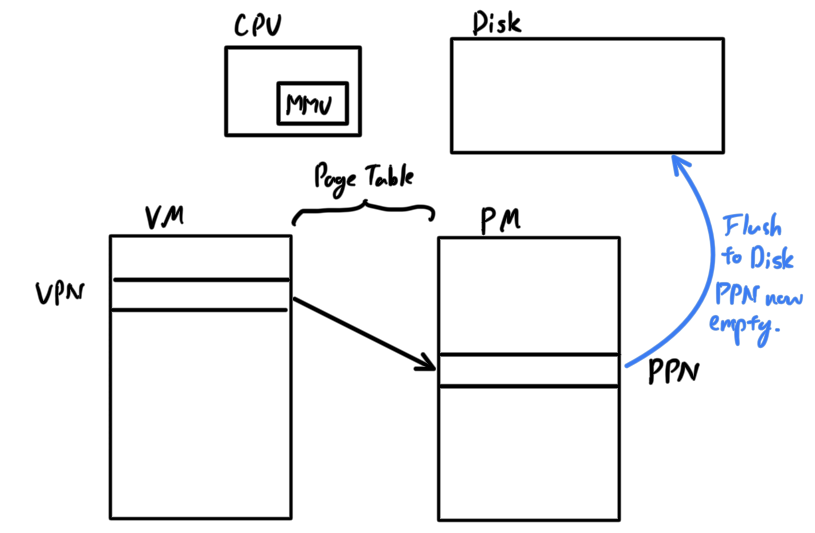
\includegraphics[scale=0.4]{img/swap.png}
        \caption{Swapping out physical pages to disk.} 
        \label{fig:swap}
      \end{figure}
      This allows us to abstract software into having almost infinite memory. Another important property is that swapping is \textbf{write-back} rather than write-through. We really don't want to write to disk every time we modify memory, so some thing may never end up on the disk (e.g. stack for short-lived processes). This is why when we open a file in C or Python, you may have to call \texttt{close()} since that will flush the memory to disk. 
    \end{definition}

    \begin{example}[Page Fault] 
      When we swap out a physical page to disk, the physical page is now empty and accessing the virtual memory at this page table will cause a page fault. Say, when we want to write to a memory address that is swapped into the disk. The following will happen. 
      \begin{enumerate}
        \item You execute code normally in user mode. 
        \item Then you try to write to a memory address that is swapped out, say through a \texttt{mov} operation. Say it is the following assembly code. 

          \begin{lstlisting}
            80483b7: c7 05 10 9d 04 08 0d          movl $0x0,0x8049d10  
          \end{lstlisting}
          This raises a page fault, an exception, and so the OS goes into kernel mode. 
        \item The kernel then finds the location of this physical page in the disk. The implementation is OS-specific (e.g. you can store some metadata). 
        \item Then it must copy the page back from disk into memory, and it may also have to swap out some other physical page to disk to make space if needed.  
        \item Then the OS goes back into user mode, which now has access to the relevant memory in disk. 
      \end{enumerate}
      Ultimately, the moving operation is called twice. The first time it fails in user mode, and the second time (after the kernel mode, but now back to user mode) it succeeds. Note that this is different from a system call, which returns back to the \textit{next} instruction. This call returns to the current instruction. 
    \end{example}

    \begin{definition}[Page Sharing]
      This also makes protection and sharing to be quite nice. Given two virtual pages $VP_1$ and $VP_2$, owned by two different processes, we can have them share information by mapping to the same physical page $PP$. 
      \begin{table}[H] 
        \centering 
        \begin{tabular}{|c|c|c|c|}
        \hline
        \textbf{Section} & \textbf{Read} & \textbf{Write} & \textbf{Execute} \\
        \hline
        Stack & 1 & 1 & 0 \\
        \hline
        Heap & 1 & 1 & 0 \\
        \hline
        Static Data & 1 & 1 & 0 \\
        \hline
        Literals/const & 1 & 0 & 0 \\
        \hline
        Instructions & 1 & 0 & 1 \\
        \hline
        \end{tabular}
        \caption{Permissions for different sections of virtual memory.}
      \end{table}
    \end{definition}

    \begin{example}[Page Sharing Between Two Applications]
      Furthermore, we can set process 1 to have only read permissions and process 2 to have read/write permissions. Therefore, say Google Chrome (process 2) can write your password into some memory, and then Slack (process 1) can read it, copy it into the CPU, and do stuff with it. 
      \begin{figure}[H]
        \centering 
        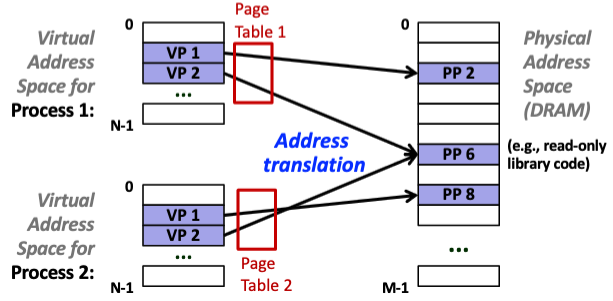
\includegraphics[scale=0.4]{img/vm_sharing.png}
        \caption{Sharing of data between two processes.} 
        \label{fig:vm_sharing}
      \end{figure}
    \end{example}

    Now that we see how memory is swapped in the backend, we can see why larger memory can sometimes mean faster programs and why thrashing occurs. 

    \begin{definition}[Thrashing]
      The set of virtual pages that a program is ``actively'' accessing at any point in time is called its \textbf{working set}. 
      \begin{enumerate}
        \item If the working set of one process is less than physical memory, then there is good performance for one process. 
        \item If the working set of all processes is greater than physical memory, then we have \textbf{thrashing}, which is a performance meltdown where pages are swapped between memory and disk continuously, and the CPU is always waiting or paging. 
      \end{enumerate}
    \end{definition}

    \begin{example}[Computation Exercise]
      Suppose that you have 16 KiB pages, 48-bit virtual addresses, and 16 GiB physical memory. How many bits wide are the following fields? 
      \begin{enumerate}
        \item Virtual page number : $48 - 14 = 34$ bits.
        \item Virtual page offset : 16 KiB is $2^{14}$ bytes, so we need $14$ bits.
        \item Physical page number : 16 GiB is $2^{34}$ bytes, so we need $34 - 14 = 20$ bits.
        \item Physical page offset : 16 KiB is $2^{14}$ bytes, so we need $14$ bits.
      \end{enumerate}
      Furthermore, we have 
      \begin{figure}[H]
        \centering 
        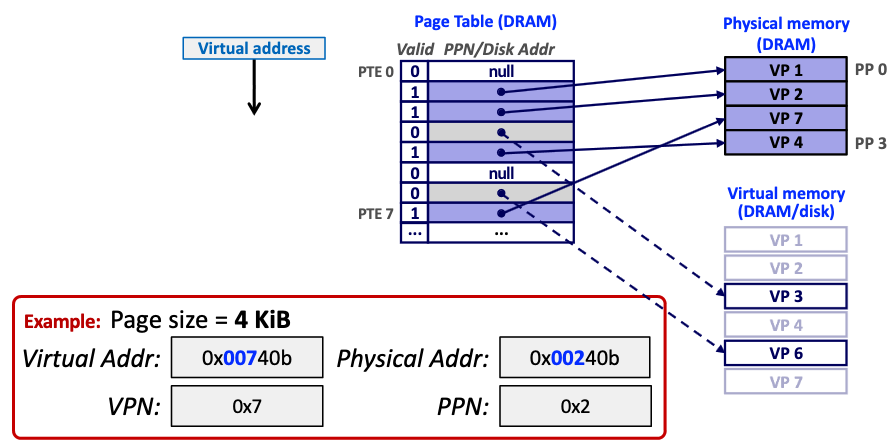
\includegraphics[scale=0.4]{img/page_example.png}
        \caption{Given the virtual address, we can figure out the physical address, VPN, and PPN easily. } 
        \label{fig:page_example}
      \end{figure}
    \end{example}

\section{Filesystems}

  Before we get into anything, even the loading of the firmware or the operating system kernel, we must talk about the hardware and how a computer stores data. Data, whether it is in memory or some disk, is just a bunch of sequences of bits. A \textbf{drive} is a physical device that can store data. A \textbf{partition} is a logical division of a drive, and a \textbf{filesystem} is a way to organize data on a drive. For example, if I have a 1TB SSD, I can run it as a single partition, or I can divide it into two partitions, one for a Windows operating system and another for a Linux operating system. A filesystem is a bit more confusing, so here are some examples. 

  \begin{example}[Linux Filesystems]
    Listed. 
    \begin{enumerate}
      \item \textbf{ext4}: The most common filesystem for Linux. 
      \item \textbf{XFS}: Designed for high performance and scalability, often used in enterprise environments for large-scale storage.
      \item \textbf{btrfs}: A modern filesystem that offers advanced features like snapshots, dynamic inode allocation, and integrated device management for better data reliability and performance. 
      \item \textbf{zfs}: Originally developed by Sun Microsystems for Solaris, ZFS is known for its data integrity, support for enormous storage capacities, and features like snapshots, copy-on-write, and built-in data compression.
    \end{enumerate}
  \end{example}

  \begin{example}[Windows Filesystems]
    Listed. 
    \begin{enumerate} 
      \item \textbf{NTFS (New Technology File System)}: The standard filesystem for Windows operating systems, supporting file permissions, encryption, and large file sizes.
      \item \textbf{FAT32 (File Allocation Table 32)}: An older filesystem with wide compatibility across different operating systems, including Windows, macOS, and various Linux distributions, though it has limitations on file and partition sizes.
      \item \textbf{exFAT (Extended File Allocation Table)}: Designed to be a lightweight filesystem similar to FAT32 but without its limitations, exFAT is used for flash drives and external hard drives due to its support for larger files and compatibility.
    \end{enumerate}
  \end{example}

  \begin{example}[MacOS Filesystems]
    Listed. 
    \begin{enumerate}
      \item \textbf{APFS (Apple File System)}: The default filesystem for macOS, iOS, and other Apple operating systems since 2017, designed for SSDs and featuring strong encryption, space sharing, and fast directory sizing.
      \item \textbf{HFS+ (Hierarchical File System Plus)}: Also known as Mac OS Extended, it was the primary filesystem for Mac computers before APFS, supporting journaling for data integrity.
    \end{enumerate}
  \end{example}

  When your computer boots up, it needs to know where to find the operating system kernel. This is done by mounting the filesystems. The \textbf{mount point} is the directory where the filesystem is attached to the system. The \textbf{root filesystem} is the filesystem that contains the operating system kernel.

  Depending on your hardware specs, you may have multiple drives. To list all drives and their partitions, run \textbf{lsblk}. The type determines whether it is a disk or a partitions, and the mountpoints determine where the partitions are mounted. Furthermore, the \texttt{RO} indicates whether this is a HDD (1) or SSD (0). 

  \begin{figure}[hbt!]
    \centering 
    \begin{lstlisting} 
      NAME        MAJ:MIN RM   SIZE RO TYPE MOUNTPOINTS
      zram0       254:0    0     4G  0 disk [SWAP]
      nvme0n1     259:0    0 953.9G  0 disk 
        nvme0n1p1 259:1    0   240M  0 part 
        nvme0n1p2 259:2    0   128M  0 part 
        nvme0n1p3 259:3    0 309.4G  0 part 
        nvme0n1p4 259:4    0   990M  0 part 
        nvme0n1p5 259:5    0  16.7G  0 part 
        nvme0n1p6 259:6    0   1.4G  0 part 
        nvme0n1p7 259:7    0   500M  0 part /boot
        nvme0n1p8 259:8    0   4.7G  0 part [SWAP]
        nvme0n1p9 259:9    0 619.9G  0 part /
    \end{lstlisting}
    \caption{This is the following output on my personal computer. } 
    \label{fig:lsblk}
  \end{figure}
    
  The \textbf{swap} partition is a special type of partition that is used as a temporary storage area for the operating system. It is used when the system runs out of RAM. 

  For a more detailed view on what the partitions consist of, you can run \textbf{fdisk -l}.
  \begin{lstlisting} 
    Disk /dev/nvme0n1: 953.87 GiB, 1024209543168 bytes, 2000409264 sectors
    Disk model: PM9A1 NVMe Samsung 1024GB               
    Units: sectors of 1 * 512 = 512 bytes
    Sector size (logical/physical): 512 bytes / 512 bytes
    I/O size (minimum/optimal): 512 bytes / 512 bytes
    Disklabel type: gpt
    Disk identifier: 26D88CE9-B388-4CF1-856C-14D5EEB0C143

    Device              Start        End    Sectors   Size Type
    /dev/nvme0n1p1       2048     493567     491520   240M EFI System
    /dev/nvme0n1p2     493568     755711     262144   128M Microsoft reserved
    /dev/nvme0n1p3     755712  649658367  648902656 309.4G Microsoft basic data
    /dev/nvme0n1p4 1960380416 1962407935    2027520   990M Windows recovery environment
    /dev/nvme0n1p5 1962407936 1997441023   35033088  16.7G Windows recovery environment
    /dev/nvme0n1p6 1997443072 2000377855    2934784   1.4G Windows recovery environment
    /dev/nvme0n1p7  649658368  650682367    1024000   500M EFI System
    /dev/nvme0n1p8  650682368  660447231    9764864   4.7G Linux swap
    /dev/nvme0n1p9  660447232 1960380415 1299933184 619.9G Linux filesystem
  \end{lstlisting}

  As you can see here, my single disk has 9 partitions. 
  \begin{enumerate} 
    \item The first EFI system (1) or the Microsoft reserved (2) partition contains the Windows operating system kernel. 
    \item The Microsoft basic data (3) partition contains the Windows files.
    \item  The Windows recovery environment (4, 5, 6) is a partition that contains the Windows recovery environment, which are partitions set aside by the manufacturer to hold an image of your system before it was shipped from the factory. 
    \item The EFI system (7) partition contains the Linux operating system kernel, which is required to load the operating system. 
    \item The Linux swap (8) partition is a partition that contains the Linux swap. 
    \item The Linux filesystem (9) is a partition that contains the actual Linux operating system itself, along with all your files.
  \end{enumerate}


  \subsection{Mounting} 

    You can further go into the \texttt{/dev} directory to see the devices that are mounted, e.g. the \texttt{/dev/nvme0n1p9} is the device that is mounted on the root directory, and most of these files are either device files (which are special files that provide an interface to hardware devices, allowing software and users to interact with them as if they were normal files) or symlinks.

    The \textbf{mount} command is used to attach a filesystem to the system's directory tree. The \textbf{umount} command is used to detach a filesystem from the system's directory tree. 

    \begin{enumerate}
      \item \textbf{Mounting a filesystem}: The general syntax is \texttt{mount -t type device dir}. For example, to mount the \texttt{/dev/nvme0n1p9} to the root directory, you can run \texttt{mount -t ext4 /dev/nvme0n1p9 /mnt}. 
      \item \textbf{Unmounting a filesystem}: The general syntax is \texttt{umount dir}. For example, to unmount the root directory, you can run \texttt{umount /mnt}. 
    \end{enumerate}

    When the computer boots up, it must automatically mount the specific filesystems. This is configured in the \textbf{fstab} file. 

    \begin{definition}[fstab]
      The \textbf{fstab} file is a system configuration file that contains information about filesystems. It is located at \texttt{/etc/fstab}. It is used to define how disk partitions, various other block devices, or remote filesystems should be mounted into the filesystem. 
      Each line in the file contains six fields, separated by whitespace. The fields include: 
      \begin{enumerate} 
        \item \textbf{Filesystem}: The block device or remote filesystem to be mounted. This can be the UUID (Universally Unique Identifier), the label, or the traditional device name (like /dev/sda1) that specifies which device or partition is being referred to.
        \item \textbf{Mount Point}: The directory where the filesystem should be mounted. 
        \item \textbf{Type}: The type of the filesystem, e.g. ext4, vfat, swap, etc.
        \item \textbf{Options}: Mount options for the filesystem, e.g. \texttt{rw} for read-write, \texttt{ro} for read-only, \texttt{noexec} to prevent execution of binaries, etc.
        \item \textbf{Dump}: A number used by the \textbf{dump} command to determine whether the filesystem should be backed up. It is often set to $0$ to disable backups. 
        \item \textbf{Pass}: A number used by the \textbf{fsck} command to determine the order in which filesystems should be checked. Root filesystems should have this set to 1, and other filesystems should either be 2 (to check after the root) or 0 (to disable checking). 
      \end{enumerate}
    \end{definition}
    \begin{figure}[hbt!]
      \centering 
      \begin{lstlisting} 
        # Static information about the filesystems.
        # See fstab(5) for details.

        # <file system> <dir> <type> <options> <dump> <pass>
        # /dev/nvme0n1p9
        UUID=abcfef03-bfae-4d1f-b463-fd6538f18a41	/ ext4 rw,relatime 0 1
        # /dev/nvme0n1p7
        UUID=150D-7A67 /boot vfat rw,relatime,fmask=0077,dmask=0077,codepage=437,
            iocharset=ascii,shortname=mixed,utf8,errors=remount-ro	0 2
        # /dev/nvme0n1p8
        UUID=5c191f65-b016-475d-b04a-5b7c89bda31d	none swap defaults 0 0
      \end{lstlisting}
      \caption{My personal fstab file.} 
      \label{fig:fstab}
    \end{figure}

    \subsubsection{Mounting a Remote Disk} 

      It is actually possible to mount a folder on a server into your local machine. To do this, you use \textbf{sshfs} to mount a remote directory over SSH. The general syntax is \texttt{sshfs user@host:/remote/dir /local/dir} to mount and \texttt{fusermount -u /local/dir} to unmount. 

  \subsection{Maintence} 

    \subsubsection{SSD}

      As soon as your write or delete bits from the SSD (e.g. when you're deleting a file), it degrades the speed of the read/write. To alleviate the effects, you can use TRIM, which is a command that allows the operating system to inform the SSD which blocks of data are no longer considered in use and can be wiped internally. It can be downloaded as a part of the \texttt{util-linux} package, which provides the systemd services \textbf{fstrim.timer} and \textbf{fstrim.service}. It is recommended to use weekly trims rather than continuous trims. 

    \subsubsection{Filesystem} 

      Occasionally, you may have a corrupt partitions, whether it is your boot or root directory. In this case, you should use the \textbf{fsck} command to check and repair a filesystem. The general steps are: 
      \begin{enumerate} 
        \item unmount the specific partition you want (identified with \textbf{lsblk}) using \texttt{sudo umount /dev/partition}. 
        \item run \texttt{sudo fsck -t type device} (or for specific filesystem types like vfat you can be a bit more specific by running \texttt{sudo fsck.vfat /dev/partition}) to check the filesystem and fix any changes. 
        \item mount the specific partition back using \texttt{sudo mount /dev/partition}. 
      \end{enumerate}

  \subsection{Modifying Partitions} 
    
    Modifying partitions require specialized software. Partitioning can be done using two main partitioning schemes \textbf{GPT} (the modern one) and \textbf{MBR} (legacy). The \textbf{parted} utility gives detailed info on your partitions. To see which scheme you have, just run \texttt{sudo parted -l}, where the output can be shown in Figure \ref{fig:parted}. 

    \begin{figure}[hbt!]
      \centering 
      \begin{lstlisting} 
        Model: PM9A1 NVMe Samsung 1024GB (nvme)
        Disk /dev/nvme0n1: 1024GB
        Sector size (logical/physical): 512B/512B
        Partition Table: gpt
        Disk Flags: 

        Number  Start   End     Size    File system     Name                          Flags
         1      1049kB  253MB   252MB   fat32           EFI system partition          boot, esp
         2      253MB   387MB   134MB                   Microsoft reserved partition  msftres
         3      387MB   333GB   332GB   ntfs            Basic data partition          msftdata
         7      333GB   333GB   524MB   fat32                                         boot, esp
         8      333GB   338GB   5000MB  linux-swap(v1)                                swap
         9      338GB   1004GB  666GB   ext4
         4      1004GB  1005GB  1038MB  ntfs                                          hidden, diag
         5      1005GB  1023GB  17.9GB  ntfs                                          hidden, diag
         6      1023GB  1024GB  1503MB  ntfs                                          hidden, diag


        Model: Unknown (unknown)
        Disk /dev/zram0: 4295MB
        Sector size (logical/physical): 4096B/4096B
        Partition Table: loop
        Disk Flags: 

        Number  Start  End     Size    File system     Flags
         1      0.00B  4295MB  4295MB  linux-swap(v1) 
      \end{lstlisting}
      \caption{Output of \texttt{sudo parted -l} on my own machine. } 
      \label{fig:parted}
    \end{figure}

    It is important to know which partition scheme you should use. 
    \begin{enumerate} 
      \item To dual-boot with Windows (both 32-bit and 64-bit) using Legacy BIOS, the MBR scheme is required.
      \item To dual-boot Windows 64-bit using UEFI mode instead of BIOS, the GPT scheme is required.
      \item If you are installing on older hardware, especially on old laptops, consider choosing MBR because its BIOS might not support GPT.
      \item If you are partitioning a disk that is larger than 2TB, you need to use GPT.
      \item It is recommended to always use GPT for UEFI boot, as some UEFI implementations do not support booting to the MBR while in UEFI mode.
    \end{enumerate}

\section{I/O Systems}

\section{Storage Management}

\section{Virtualization}


\section{Firmware} 

    Let us go through the steps of a booting (bootstrapping) process. Administrators have little direct, interactive control over most of the steps required to boot a system, but they can modify bootstrap configurations by editing config files or system startup scripts. 

    \begin{enumerate}
      \item \textbf{Power On}: You power on the machine. 
      \item \textbf{Load firmware from NVRAM}: You want to be able to identify the specific piece of hardware to load your operating system in. The firmware is a permanent piece of software that does this. 
      \item \textbf{Probe for hardware}: We look for hardware that is on the computer. 
      \item \textbf{Select boot device (disk, network, etc.)}: We select the storage device that we want to load the operating system on. 
      \item \textbf{Identify EFI system partition}: 
      \item \textbf{Load boot loader (e.g. GRUB)}: A software that allows you to identify and load the proper OS kernel is provided. 
      \item \textbf{Determine which kernel to boot}: You choose which kernel you want to load.  
      \item \textbf{Load kernel}: The OS kernel is identified and loaded into the boot device. 
      \item \textbf{Instantiate kernel data structure}: 
      \item \textbf{Start init/systemd as PID 1}: 
      \item \textbf{Exectute startup scripts}:
      \item \textbf{Running system}: You now have a running system! 
    \end{enumerate}

    Right above the hardware, the \textbf{system firmware}, is a piece of software that is executed whenever the computer boots up. 
    \begin{enumerate} 
      \item \textbf{Power Supply Activation}: Once the computer is turned on, the power supply begins to provide electricity to the system's components. One of the first signals generated is the "Power Good" signal, indicating that the power supply is stable and at the correct voltages. 
      \item \textbf{CPU Reset}: Upon receiving the "Power Good" signal, the CPU resets and starts its operations. The CPU is designed to start executing instructions from a predefined memory address, which is hardwired into the CPU. This address, stored in ROM, contains the starting point of the firmware.\textbf{Read Only Memory} is simply another type of computer memory that stores permanent data and instructions for the device to start up. 
      \item \textbf{Predefined Memory Address}: For BIOS systems, the CPU begins executing code at the firmware entry point located in the system's ROM (Read-Only Memory). In UEFI systems, the process is similar, but the UEFI firmware provides more functionalities and a more flexible pre-boot environment.
      \item \textbf{POST (Power on Self Test)}: The firmware conducts a series of diagnostic tests to ensure that essential hardware components like RAM, storage devices, and input/output systems are functioning correctly. This stage is critical for verifying system integrity before loading the operating system.
    \end{enumerate}

    To be honest, there is not a lot that the user can control here with just software. The firmware is a permanent piece of software that is executed whenever the computer boots up, which makes it relatively safe from tampering. If your computer fails to boot up, the most fundamental reason may be a firmware problem. However, we're not screwed yet. 

    Most firmware offers a user interface which can be accessed by pressing the F2, F11, F12, or some combination of magic keys at the instant the system first powers on. Depending on what computer model you have, you may have some control of basic functionalities. 
    
    \begin{figure}[hbt!]
      \centering 
      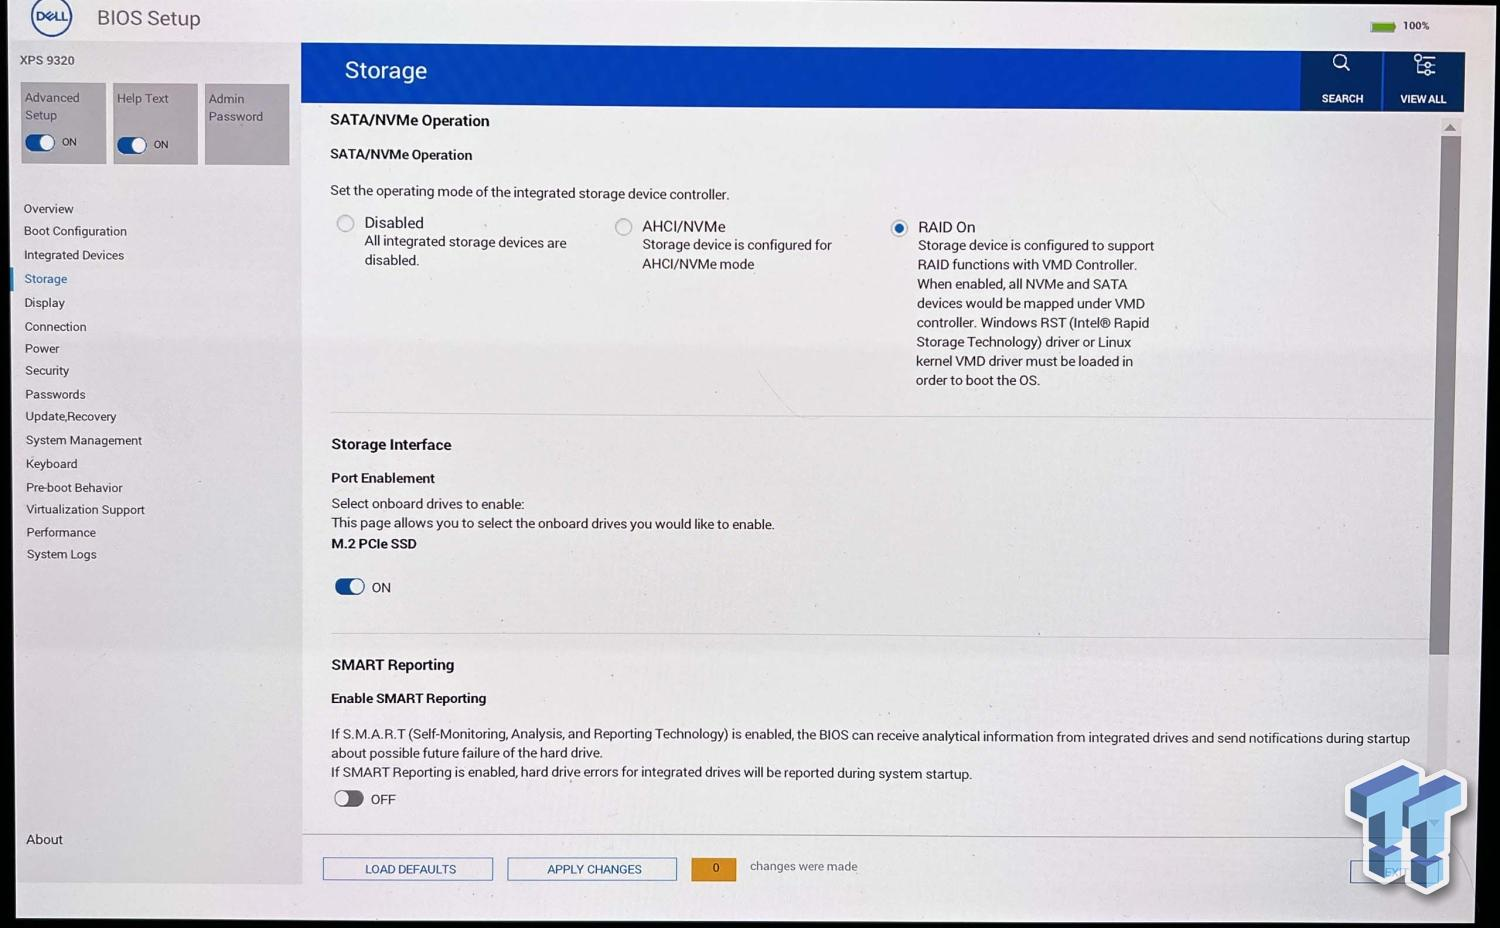
\includegraphics[scale=0.3]{img/xps_firmware.jpg}
      \caption{Firmware of Dell XPS 13 9320} 
      \label{fig:xps_firmware}
    \end{figure}

    Some important functionalities you can do with the firmware are: 
    \begin{enumerate} 
      \item Determine the boot order of the devices, usually by prioritizing a list of available options (e.g. try to boot from a DVD drive, then a USB, then the hard disk). 
      \item 
    \end{enumerate}

    The \textbf{BIOS}, which stands for \textbf{Basic Input/Output System}, has been used traditionally. It is mainly responsible for loading the bootloader. When the computer starts, it runs a \textbf{Power on Self Test (POST)} to make sure that core hardware such as the memory and hard disk is working properly. Afterward, the BIOS will check the primary hard drives' \textbf{Master Boot Record (MBR)}, which is a section on your hard drive where the bootloader is located. 

    A more formalized and modern standard called \textbf{EFI} (\textbf{Extensible Firmware Interface}) has replaced it, and it has been revised to the \textbf{UEFI} (\textbf{Unified Extensible Firmware Interface}) standard, but we can treat EFI and UEFI as equivalent in most cases. Fortunately, most UEFI systems can fall back to a legacy BIOS impelmentation if the operating system they're booting doesn't support UEFI. Since we're likely to encounter boot firmware systems, it's worthwhile to go into both of them. 

  \subsection{Updating Firmware}

    The first thing you should do when you're having trouble with firmware is use \textbf{fwupd}, which is a daemon that handles firmware updates. It is a simple daemon to allow session software to update device firmware on your local machine. Upon installation, it creates a systemd agent on \texttt{/lib/systemd/system/fwupd.service}. It does not start automatically. I have used this to update my firmware, which saved a lot of booting errors, with instructions accessed in this \href{https://wiki.archlinux.org/title/fwupd}{link}. 

  \subsection{Modifying UEFI Variables}

    You can directly examine and modify UEFI variables on a running system with the \texttt{efibootmgr} command. You get a following summary of the configuration: 
    \begin{lstlisting}
      BootCurrent: 0005
      Timeout: 0 seconds
      BootOrder: 0005,0001,0002,0000,0003,0004
      Boot0000* UEFI PM9A1 NVMe Samsung 1024GB S65VNE0R318841 1	...
      Boot0001* ubuntu	HD(1,GPT,ede98b7e-75ad-452e-ab47-3411dd6026c1,0x800,0x780...
      Boot0002* Windows Boot Manager	HD(1,GPT,ede98b7e-75ad-452e-ab47-3411dd60...
      Boot0003* Linux Firmware Updater	HD(1,GPT,ede98b7e-75ad-452e-ab47-...
      Boot0004* UEFI PM9A1 NVMe Samsung 1024GB S65VNE0R318841 1 2	PciRoot(0x0)/...
      Boot0005* Linux Boot Manager	HD(7,GPT,2d28b70f-725b-4ca3-98d4-25f5c83fc00e...
    \end{lstlisting}

    It shows you which disk you are currently booted into, the boot order that is currently configured, and information about each of the disks. You can use a GUI to do this as well. You can press a certain key when booting (F2 on my Dell XPS15 9500) to enter the \textbf{BIOS setup}. 

    \begin{figure}[H]
      \centering 
      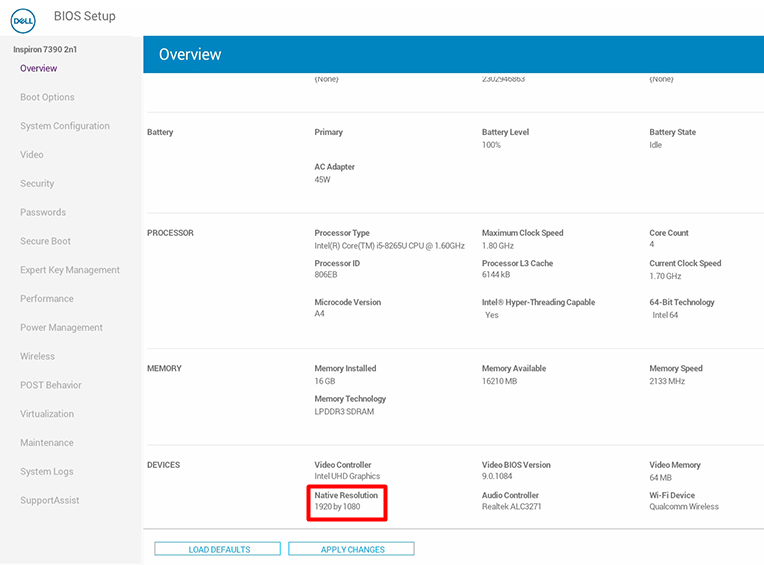
\includegraphics[scale=0.45]{img/firmware.jpeg}
      \caption{The BIOS setup can look very different depending on the computer but looks like this for me.} 
      \label{fig:bios_setup}
    \end{figure}

    From here, we can edit different settings like boot options (priority of booting OS), certain video settings, etc. 

  \subsection{Recovery Mode}

    Occasionally, you may run into problems with booting up the system. You can go into \textbf{recovery mode} by looking at the advanced options in the GRUB menu and selecting the option that literally says recovery mode. 

    \begin{center}
      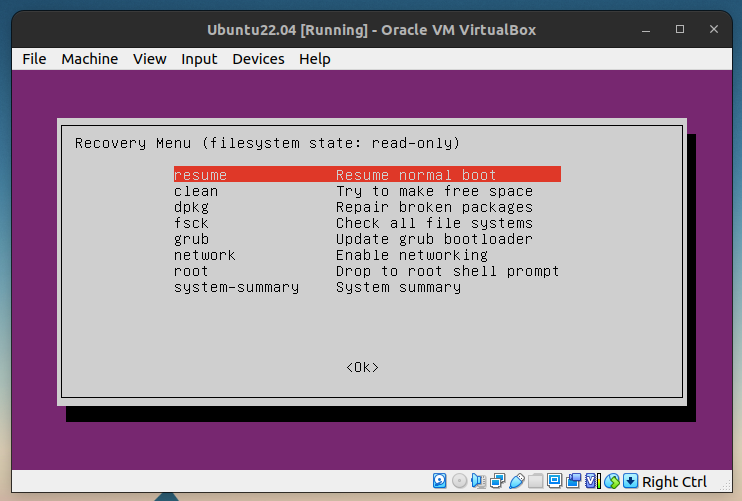
\includegraphics[scale=0.3]{img/recovery1.png}
    \end{center}

    This gives us a list of options that we can take to fix the system. Every setting except root is automatically done. The root command gives us root privileges (no sudo is needed). This also means we have full access to all files, and we may cause irreversible damage to our system if we made a mistake. If we had not enabled read/write access with "Enable networking" the filesystem will be mounted read only, and we are unable to edit files. In case we don't have access to a network, or this was not desired, we can remount our filesystem(s) giving write access with the following command:  
    \begin{lstlisting}
      mount -o rw,remount /
    \end{lstlisting}
    With editing privileges, we can hopefully better diagnose or undo our problems. Finally, from the root shell type $\texttt{exit}$ to go back to the menu. 

\section{Bootloaders} 

  Once the firmware is loaded, which probes the system to find the hardware, it must load the operating system kernel. This is the job of the boot loader.

  \begin{definition}[Boot Loader, Boot Manager]
    The \textbf{bootloader} is another critical piece of software that allows you to identify and load the proper operating system kernel. If it also provides an interactive menu with multiple boot choices, then it is often called a \textbf{boot manager}. 
  \end{definition}

  In modern systems which support UEFI (not the legacy BIOS), you must configure your partitions so that there exists an EFI partition (at \texttt{/boot}) that contains this bootloader. 

  EFI bootloaders usually have a \texttt{.efi} extension, and it is crucial that you know where the bootloaders are in your system in case they go missing or are corrupt. To see the configuration, you can run \textbf{efibootmgr} (with verbose), which gives you information on several things: 
  \begin{enumerate} 
    \item It scans the entire system for EFI bootloaders and lists them. 
    \item It lists the locations of the EFI bootloaders. It starts off which what partition they are in, and then lists the directory where the bootloader is located. \texttt{BootX64.efi} is the Windows bootloader and \texttt{grubx64.efi} is the GRUB bootloader. For example, you may have a bootloader at \texttt{(partition 7)/boot/efi/EFI/Boot/bootx64.efi}. 
    \item It lists the boot order, which is the order in which the bootloaders are loaded. In case a boot loader fails to load, the next one is loaded. Therefore, if you have an arch linux bootloader that is corrupt, and the next in line is the Windows bootloader, you will automatically boot into Windows. You can also set the boot order in the BIOS. 
  \end{enumerate}

  In case you can't boot in, you can always get an Arch ISO burned in on a thumb drive, boot into it, mount the relevant partitions containing the Arch bootloader and the root directory, and then chroot into the root directory to modify files. 

  \subsection{GRUB}

    The way that these kernels can be loaded can be configured through the bootloader, and the most popular boot manager is \textbf{GRUB}, the \textbf{Grand Unified Bootloader}. GRUB, developed by the GNU project, is the default loader on most Linux distributions. There is an old version called GRUB legacy and the more modern GRUB 2. Most people refer to GRUB 2 and simply GRUB. FreeBSD, which is another complete (non-Linux) OS, have their own boot loader, but GRUB is compatible with it. Therefore, for dual-boot or triple-boot systems that have multiple kernels, GRUB is the go-to bootloader for loading any of them. 

    \begin{figure}[H]
      \centering 
      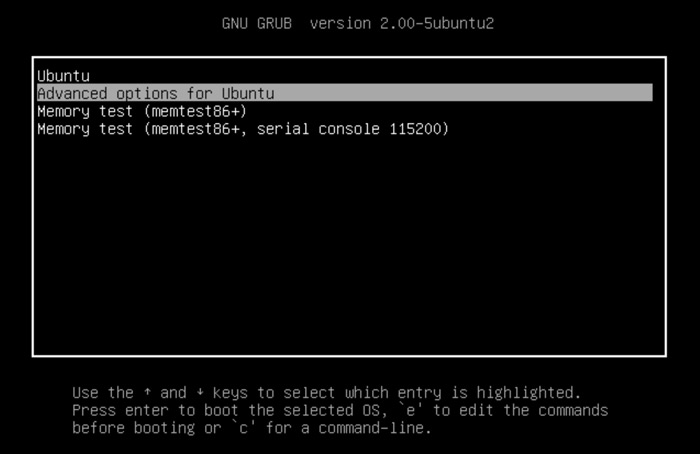
\includegraphics[scale=0.4]{img/grub2-in-ubuntu.png}
      \caption{GRUB menu on my screen. Ubuntu does not display the GRUB menu by default. To see GRUB during boot you need to press the right-hand SHIFT key during boot. } 
      \label{fig:grub}
    \end{figure}


    As a critical piece of software, we would expect its configuration files to be in the NVRAM, but GRUB understands most of the filesystems in common use and can find its way into the root filesystem on its own. Therefore, we can read its configuration from a regular text file, kept in \texttt{/boot/grub/grub.cfg}. Changing the boot configuration is as simple as updating the \texttt{grub.cfg} file, but it is not advised to edit it directly. Rather, we can edit the $\texttt{/etc/default/grub}$ file and run $\texttt{sudo update-grub}$ to that the changes are written to $\texttt{grub.cfg}$ automatically.  


\end{document}

